% **************************************************
% Document Class Definition
% **************************************************
\documentclass[%
	paper=A4,					% paper size --> A4 is default in Germany
	twoside=true,				% onesite or twoside printing
	openright,					% doublepage cleaning ends up right side
	parskip=full,				% spacing value / method for paragraphs
	chapterprefix=true,			% prefix for chapter marks
	11pt,						% font size
	headings=normal,			% size of headings
	bibliography=totoc,			% include bib in toc
	listof=totoc,				% include listof entries in toc
	titlepage=on,				% own page for each title page
	captions=tableabove,		% display table captions above the float env
	draft=false,				% value for draft version
]{scrreprt}%

% **************************************************
% Debug LaTeX Information
% **************************************************
%\listfiles

% **************************************************
% Information and Commands for Reuse
% **************************************************
\newcommand{\thesisTitle}{The Clean Thesis Style}
\newcommand{\thesisName}{Ricardo Langner}
\newcommand{\thesisSubject}{Documentation}
\newcommand{\thesisDate}{August 26, 2015}
\newcommand{\thesisVersion}{My First Draft}

\newcommand{\thesisFirstReviewer}{Jane Doe}
\newcommand{\thesisFirstReviewerUniversity}{\protect{Clean Thesis Style University}}
\newcommand{\thesisFirstReviewerDepartment}{Department of Clean Thesis Style}

\newcommand{\thesisSecondReviewer}{John Doe}
\newcommand{\thesisSecondReviewerUniversity}{\protect{Clean Thesis Style University}}
\newcommand{\thesisSecondReviewerDepartment}{Department of Clean Thesis Style}

\newcommand{\thesisFirstSupervisor}{Jane Doe}
\newcommand{\thesisSecondSupervisor}{John Smith}

\newcommand{\thesisUniversity}{\protect{Clean Thesis Style University}}
\newcommand{\thesisUniversityDepartment}{Department of Clean Thesis Style}
\newcommand{\thesisUniversityInstitute}{Institut for Clean Thesis Dev}
\newcommand{\thesisUniversityGroup}{Clean Thesis Group (CTG)}
\newcommand{\thesisUniversityCity}{City}
\newcommand{\thesisUniversityStreetAddress}{Street address}
\newcommand{\thesisUniversityPostalCode}{Postal Code}

%\newcommand{\forcenewpage}{\clearpage \newpage \mbox{~} \clearpage \newpage}
\newcommand{\forcenewpage}{\clearpage \mbox{~}}

% --------------------------
% new commands
% --------------------------
\newcommand{\CC}{\ensuremath{\mathbb{C}} }
\newcommand{\NN}{\ensuremath{\mathbb{N}} }
\newcommand{\RR}{\ensuremath{\mathbb{R}} }
\newcommand{\QQ}{\ensuremath{\mathbb{Q}} }
\newcommand{\EE}{\ensuremath{\mathbb{E}} }
\newcommand{\PP}{\ensuremath{\mathbb{P}} }
\newcommand{\noi}{\noindent}
\newcommand{\II}{\mbox{\large 1\hskip -0,353em 1}}
\newcommand{\dps}{\displaystyle}
\newcommand{\ms}{\medskip}
\newcommand{\itb}{\ms\item[$\bullet$]}
\newcommand{\itm}{\ms\item}
\newcommand{\pkg}[1]{{\normalfont\fontseries{b}\selectfont #1}}
\newcommand{\proglang}[1]{\textsf{#1}}
\newcommand{\code}[1]{\mbox{\texttt{#1}}}
\newcommand{\MN}{\mathcal{N}}
\newcommand{\MM}{\mathcal{M}}
\newcommand{\FF}{\mathcal{F}}
\newcommand{\GG}{\mathcal{G}}
\newcommand{\HH}{\mathcal{H}}
\newcommand{\LL}{\mathcal{L}}
\newcommand{\AT}{\mathcal{A}}


% **************************************************
% Load and Configure Packages
% **************************************************
\usepackage[utf8]{inputenc}		% defines file's character encoding
\usepackage[english]{babel} % babel system, adjust the language of the content
\usepackage[					% clean thesis style
	figuresep=colon,%
	sansserif=false,%
	hangfigurecaption=false,%
	hangsection=true,%
	hangsubsection=true,%
	colorize=full,%
	colortheme=bluemagenta,%
	bibsys=bibtex,%
	bibfile=bib-refs,%
	bibstyle=alphabetic,%
]{cleanthesis}

% --------------------------
% packages
% --------------------------
\usepackage{amssymb,amsfonts,amsmath}

\usepackage{graphicx}

\def\proof{\noindent \textbf{\emph{\textbf{Proof}.$\,$}}}
\def\finproof {\hfill $\Box$ \vskip 5 pt }


\hypersetup{					% setup the hyperref-package options
	pdftitle={\thesisTitle},	% 	- title (PDF meta)
	pdfsubject={\thesisSubject},% 	- subject (PDF meta)
	pdfauthor={\thesisName},	% 	- author (PDF meta)
	plainpages=false,			% 	-
	colorlinks=false,			% 	- colorize links?
	pdfborder={0 0 0},			% 	-
	breaklinks=true,			% 	- allow line break inside links
	bookmarksnumbered=true,		%
	bookmarksopen=true			%
}

% **************************************************
% Document CONTENT
% **************************************************
\begin{document}

% --------------------------
% rename document parts
% --------------------------
%\renewcaptionname{ngerman}{\figurename}{Abb.}
%\renewcaptionname{ngerman}{\tablename}{Tab.}
\renewcaptionname{english}{\figurename}{Fig.}
\renewcaptionname{english}{\tablename}{Tab.}

% --------------------------
% Front matter
% --------------------------
\pagenumbering{roman}			% roman page numbing (invisible for empty page style)
\pagestyle{empty}				% no header or footers
% !TEX root = ../thesis-example.tex
%
% ------------------------------------  --> cover title page
\begin{titlepage}
\setlength{\parindent}{0pt}
\thispagestyle{empty}


\begin{center}

\includegraphics[height=1.75cm]{gfx/logo}
\end{center}


\fontsize{10pt}{12pt}\selectfont
N\textsuperscript{o} d'ordre NNT : xxx

\vspace{0.1cm}

\begin{center}
\fontsize{13pt}{15pt}\selectfont
\textbf{\uppercase{Thèse de doctorat de l'universit\'e de Lyon}}\\
\fontsize{11pt}{13pt}\selectfont
oper\'ee au sein de\\
\textbf{l'Universit\'e Claude Bernard Lyon 1}

\vspace{0.2cm}

\textbf{Ecole Doctorale ED SEG\\% rectifier le numero d'accreditation
EA n°2429}% nom complet de l'ecole doctorale

\vspace{0.1cm}

\textbf{Specialit\'e de doctorat : Actuariat\\
Discipline : Sciences de Gestion} % eventuellement

\vspace{0.1cm}

Soutenue publiquement le 05/07/2018, par :\\
\fontsize{14pt}{16pt}\selectfont
\textbf{Thierry Moudiki Ndoumbe}

\vspace{0.1cm} % adapter à la longueur du titre

\rule[20pt]{\textwidth}{0.5pt}

\fontsize{20pt}{25pt}\selectfont
\textbf{Interest rates modeling for insurance - interpolation, extrapolation, and forecasting}

\rule{\textwidth}{0.5pt}

\vspace{0.1cm} % adapter à la longueur du titre
\end{center}

\fontsize{11pt}{13pt}\selectfont
Devant le jury compos\'e de :
\medskip

\fontsize{9pt}{11pt}\selectfont

Nom Prenom, grade/qualit\'e, \'etablissement/entreprise \hfill Pr\'esident(e)

\medskip

Franck Moraux, Professeur des universit\'es, Universit\'e de Rennes I \hfill  Rapporteur(e)

Donatien Hainaut,  Professeur des universit\'es, Universit\'e Catholique de Louvain \hfill Rapporteur(e)

Diana Dorobantu, Maitre de Conf\'erences, ISFA, Universit\'e Lyon I \hfill Examinatrice

Armelle Guillou, Professeure des universit\'es, Universit\'e de Strasbourg \hfill Examinatrice

Florence Picard, Pr\'esidente de la commission scientifique, Institut des actuaires \hfill Examinatrice

St\'ephane Loisel, Professeur des universit\'es, ISFA, Universit\'e Lyon I \hfill Examinateur/trice

\medskip

Fr\'ed\'eric Planchet, Professeur des universit\'es, ISFA, Universit\'e Lyon I \hfill Directeur de thèse

Areski Cousin, Professeur des universit\'es, Universit\'e de Strasbourg \hfill Co-directeur de thèse % le cas echeant

\newpage
%\fontsize{12pt}{14pt}\selectfont   % si le document general n'est pas en police 11pt, decommenter et preciser la taille utilisee
% Suite du manuscrit
\end{titlepage}


% ------------------------------------  --> main title page
% \begin{titlepage}
% 	\pdfbookmark[0]{Titlepage}{Titlepage}
% 	\tgherosfont
% 	\centering
%
% 	{\Large \thesisUniversity} \\[4mm]
% 	
\includegraphics[width=6cm]{gfx/Clean-Thesis-Logo} \\[2mm]
% 	\textsf{\thesisUniversityDepartment} \\
% 	\textsf{\thesisUniversityInstitute} \\
% 	\textsf{\thesisUniversityGroup} \\
%
% 	\vfill
% 	{\large \thesisSubject} \\[5mm]
% 	{\LARGE \color{ctcolortitle}\textbf{\thesisTitle} \\[10mm]}
% 	{\Large \thesisName} \\
%
% 	\vfill
% 	\begin{minipage}[t]{.27\textwidth}
% 		\raggedleft
% 		\textit{1. Reviewer}
% 	\end{minipage}
% 	\hspace*{15pt}
% 	\begin{minipage}[t]{.65\textwidth}
% 		{\Large \thesisFirstReviewer} \\
% 	  	{\small \thesisFirstReviewerDepartment} \\[-1mm]
% 		{\small \thesisFirstReviewerUniversity}
% 	\end{minipage} \\[5mm]
% 	\begin{minipage}[t]{.27\textwidth}
% 		\raggedleft
% 		\textit{2. Reviewer}
% 	\end{minipage}
% 	\hspace*{15pt}
% 	\begin{minipage}[t]{.65\textwidth}
% 		{\Large \thesisSecondReviewer} \\
% 	  	{\small \thesisSecondReviewerDepartment} \\[-1mm]
% 		{\small \thesisSecondReviewerUniversity}
% 	\end{minipage} \\[10mm]
% 	\begin{minipage}[t]{.27\textwidth}
% 		\raggedleft
% 		\textit{Supervisors}
% 	\end{minipage}
% 	\hspace*{15pt}
% 	\begin{minipage}[t]{.65\textwidth}
% 		\thesisFirstSupervisor\ and \thesisSecondSupervisor
% 	\end{minipage} \\[10mm]
%
% 	\thesisDate \\
%
% \end{titlepage}


% ------------------------------------  --> lower title back for single page layout
% \hfill
% \vfill
% {
% 	\small
% 	\textbf{\thesisName} \\
% 	\textit{\thesisTitle} \\
% 	\thesisSubject, \thesisDate \\
% 	Reviewers: \thesisFirstReviewer\ and \thesisSecondReviewer \\
% 	Supervisors: \thesisFirstSupervisor\ and \thesisSecondSupervisor \\[1.5em]
% 	\textbf{\thesisUniversity} \\
% 	\textit{\thesisUniversityGroup} \\
% 	\thesisUniversityInstitute \\
% 	\thesisUniversityDepartment \\
% 	\thesisUniversityStreetAddress \\
% 	\thesisUniversityPostalCode\ and \thesisUniversityCity
% }
		% INCLUDE: all titlepages
\cleardoublepage

\pagestyle{plain}				% display just page numbers
%% !TEX root = ../thesis-example.tex
%
\pdfbookmark[0]{Abstract}{Abstract}
\chapter*{Abstract}
\label{sec:abstract}
\vspace*{-10mm}

\blindtext

\vspace*{20mm}

{\usekomafont{chapter}Abstract (different language)}\label{sec:abstract-diff} \\

\blindtext
		% INCLUDE: the abstracts (english and german)
%\cleardoublepage
%
%% !TEX root = ../thesis-example.tex
%
\pdfbookmark[0]{Acknowledgement}{Acknowledgement}
\chapter*{Acknowledgement}
\label{sec:acknowledgement}
\vspace*{-10mm}

Thank you, to those who made this possible.
 % INCLUDE: acknowledgement
%\cleardoublepage
%
\setcounter{tocdepth}{2}		% define depth of toc
\tableofcontents				% display table of contents
\cleardoublepage

% --------------------------
% Body matter
% --------------------------
\pagenumbering{arabic}			% arabic page numbering
\setcounter{page}{1}			% set page counter
\pagestyle{maincontentstyle} 	% fancy header and footer

%% !TEX root = ../thesis-example.tex
%

\chapter{Introduction}
\label{sec:intro}

\section{Motivation and Problem Statement (French version)}

L'ORSA (Own Risk Solvency and Assessment) est un ensemble de règles définies par la directive européenne Solvabilit\'e II, destiné à servir d'outil d'aide à la décision et d'analyse stratégique des risques. Dans le cadre de l'ORSA, les compagnies d'assurance doivent évaluer leur solvabilité future de façon continue et prospective. Et pour ce faire, elles doivent notamment obtenir des projections probabilistes de leur bilan (actif et passif) sur un certain horizon temporel.   

Dans ce travail de thèse, nous nous focalisons sur l'actif; la prévision des valeurs futures des actifs. Nous traitons plus précisément des taux d'intérêts; de la construction, de l'extrapolation, et des prévisions envisagées dans le futur pour la courbe de taux d'intérêt. Les techniques présentées sont essentiellement basées sur des méthodes d'apprentissage statistique.    

Nous parlerons généralement dans le texte de \textit{courbe de taux}, mais il s'agit en fait  de courbes de facteurs d'actualisation sans risque de défaut de contrepartie. Le risque de défaut de contrepartie n'est pas explicitement traité, mais des techniques similaires à celles développées ici, peuvent être transposées à la construction de courbe de taux incorporant un risque de défaut de contrepartie.

Nous présentons dans un premier temps, une famille de courbes de facteurs d'actualisation basées sur les modèles de taux (courts) dits d'absence d'opportunité d'arbitrage ou exogènes. À une date donnée, la courbe d'actualisation est construite à l'aide de produits dérivés de taux, dont les cotations sont disponibles sur les marchés financiers pour un nombre donné de maturités. La régularité de la courbe obtenue est également paramétrable, en fonction du résultat recherché par l'utilisateur. Nous montrons comment cette courbe de facteurs d'actualisation, obtenue à une date donnée, peut être extrapolée au-delà des maturités disponibles sur les marchés, et comment les courbes construites à différentes dates dans le temps, peuvent être utilisées pour obtenir des prévisions de taux d'intérêts dans le futur.  Pour ce dernier point portant sur la prévision, des techniques basées sur l'\textbf{analyse en composantes principales (ACP) fonctionnelle} sont appliquées aux paramètres du modèle. 

Nous présentons ensuite un modèle de prévision simultanée de séries temporelles multivariées, basé sur des réseaux de neurones dits \textbf{Random Vector Functional Link (RVFL) networks}. Les RVFL ont été utilisés avec succès par le passé, pour des problèmes de régression, de classification, et de prévision de séries temporelles univariées. La nouveauté ici, est de les appliquer à des séries temporelles multivariées avec plusieurs contraintes de régularisation sur les paramètres, et des variables explicatives quasi-aléatoires. Les exemples d'application portent sur la prévision de courbes de facteurs d'actualisation. Le modèle ainsi obtenu est un modèle robuste, notamment grâce à ses paramètres de régularisation, et on montre qu'il obtient de très bonnes performances quand il est comparé à des modèles similaires. Il peut également être utilisé dans le cadre de \textit{stress tests}. 

Dans le chapitre 4, des méthodes d'apprentissage dites ensemblistes sont appliquées à la prévision simultanée de taux d'intérêts, avec d'autres variables macroéconomiques telles que l'inflation. Ces méthodes ensemblistes sont construites à partir de modèles relativement plus simples; et le modèle de base utilisé ici pour la construction des ensembles est le modèle RVFL. Trois types de méthodes ensemblistes sont envisagées: \textbf{bootstrap aggregating},  \textbf{boosting}, et \textbf{stacked generalization}. On observe ici, généralement, que ces méthodes ensemblistes peuvent permettre d'obtenir des améliorations de performance par rapport aux modèles de base qui les constituent. Il est à noter que cette amélioration ne sera pas observée de façon systématique sur d'autres jeux de données. Mais ce type de modèle aura toujours un intérêt à être envisagé dans une optique d'accroissement des performances prédictives. 

Le chapitre suivant étudie l'application des méthodes d'apprentissage basées sur des noyaux (\textbf{Kernel Regularized Least Squares}, KRLS) à la prévision de courbes de taux d'intérêt. Les modèles de type KRLS expriment la variable à expliquer (ici, le taux \textit{spot}) comme une combinaison linéaire de distances entre les observations des variables explicatives. Ces méthodes sont appliquées ici, d'abord dans le contexte populaire de Nelson-Siegel dynamique qui représente la courbe de taux en fonction de trois facteurs explicatifs, puis directement aux taux \textit{spot}. Cette deuxième approche s'apparentant à des approches appliquées en géostatistique, permet d'obtenir de bonnes performances de prévision, tout en reproduisant des faits stylisés de la courbe de taux sans contrainte de forme supplémentaire.

Le dernier chapitre compare les différents modèles introduits dans les chapitres précédents. Pour ce faire, il revisite le modèle RVFL introduit aux chapitre 3, en adjoignant à ses paramètres une distribution \textit{a priori} (Gaussienne multivariée). Le modèle ainsi obtenu sert d'ingrédient de base à une méthode d'optimisation bayésienne, appliquée à la minimisation de l'erreur de validation croisée des modèles étudiés. De manière générale dans le texte et idéalement, il faudrait introduire en plus de l'erreur de validation croisée, une erreur de validation sur des données nouvelles, non encore rencontrées par les modèles étudiés.   


\section{Motivation and Problem Statement (English version)}
\label{sec:intro:motivation}

The Own Risk Solvency and Assessment (ORSA) is a set of processes defined in the European prudential directive Solvency II, that serve for decision-making and strategic analysis. In the context of ORSA, insurance companies are required to assess their solvency needs in a continuous and prospective way. For this purpose, they notably need to forecast their balance sheet -asset and liabilities- over a defined horizon.

Here, we specifically focus on the assets' forecasting part. \textbf{This thesis is about the Yield Curve, Forecasting, and Forecasting the Yield Curve}. We present a few novel techniques for the construction, the extrapolation of static curves (that is, curves which are constructed at a fixed date), and for forecasting the spot interest rates over time. Cross validation is widely used here as a measure of model performance, but ideally a validation set with unseen data could be considered. 

Throughout the text, when we say 'Yield Curve', we actually mean 'Discount curve'. That is: we ignore the counterparty credit risk, and consider that the curves are \textit{risk-free}. Though, the same techniques could be applied to construct/forecast the actual \textit{risk-free} curves and credit spreads' curves, and combine both to obtain pseudo-discount curves incorporating the counterparty credit risk. The structure of the thesis is described in section \ref{sec:intro:structure}.

\section{Thesis Structure}
\label{sec:intro:structure}

\textbf{Chapter \ref{sec:insurance_swap_curve}} \\[0.2em]

We derived a class of discount curve construction and extrapolation methods,  based on a class of interest rate models called \textit{exogenous short-rate models}. That means: constructing a static Yield Curve at a given date, by using some specific financial instruments with different maturities quoted at this date. Then, defining what are the discount rates beyond the longest maturity observed for these financial instruments. The extrapolated part of the curve is typically necessary for the pricing of long-term insurance liabilities. In the framework that we propose, Yield Curve forecasts can be obtained by using a \textbf{functional principal components analysis} on the model parameters.

\textbf{Chapter \ref{sec:rvfl_mts}} \\[0.2em]

We are interested in obtaining forecasts for multiple time series, by taking into account the potential nonlinear relationships between their observations. For this purpose, we used a specific type of regression model on an augmented dataset of lagged time series. Our model is inspired by dynamic regression models, with the response variable's lags included as predictors, and is known as \textbf{random vector functional link (RVFL) neural networks}. The RVFL neural networks have been successfully applied in the past, to solving regression and classification problems. The novelty of our approach is to apply an RVFL model to multivariate time series, under two separate regularization constraints on the regression parameters, and quasi-randomized features. The model can also be used for realizing \textit{stress tests}. 

\textbf{Chapter \ref{sec:rvfl_ensembles}} \\[0.2em]

The goal of ensemble learning is to combine two or more statistical/machine learning models - the base learners - into one, in order to obtain an ensemble model. The ensemble model is expected to have an improved out-of-sample error over the base models. We apply two popular ensemble learning methods to multiple time series forecasting: \textbf{bootstrap aggregating}, known as bagging, \textbf{boosting}, and \textbf{stacked generalization}, known as stacking. The base learners that we use, are the RVFL introduced in the previous paragraph.


\textbf{Chapter \ref{sec:discount_curve_krls}} \\[0.2em]

\textbf{Kernel regularized least squares} (KRLS) learning methods are applied to Yield Curve forecasting. Two types of formulations of the forecasting problem are tested. One relying on a popular framework called Dynamic Nelson-Siegel, and another one, in which we apply the KRLS directly to the explain the spot rates (response variable) as a function of the observation dates and time to maturities (covariates).

\textbf{Chapter \ref{sec:bayesian_rvfl}} \\[0.2em]

We present a \textbf{bayesian quasi-randomized vector functional link neural network model} (BQRVFL), with one hidden layer. It's a penalized regression model on an augmented data set, in which we assume that a prior multivariate gaussian distribution governs the regression parameters. The BQRVFL model is presented, along with the associated formulas for confidence interval around its predictions. It is then applied as a workhorse for \textbf{bayesian optimization} of machine learning cross-validation functions. The machine learning cross-validation functions that we consider are those associated to the selection of hyperparameters of RVFL (in a DNS framework, or directly applied to the spot rates' time series) and KRLS models (in a DNS framework, or directly applied to the spot rates).

 % INCLUDE: introduction
%\forcenewpage

%% !TEX root = ../thesis-example.tex
%
\chapter{Related Work}
\label{sec:related}

\cleanchapterquote{A picture is worth a thousand words. An interface is worth a thousand pictures.}{Ben Shneiderman}{(Professor for Computer Science)}

\Blindtext[2][1]

\section{Related Work Section 1}
\label{sec:related:sec1}

\Blindtext[2][2]

\section{Related Work Section 2}
\label{sec:related:sec2}

\Blindtext[3][2]

\section{Related Work Section 3}
\label{sec:related:sec3}

\Blindtext[4][2]

\section{Conclusion}
\label{sec:related:conclusion}

\Blindtext[2][1]
 % INCLUDE: related work
%\forcenewpage

%% !TEX root = ../thesis-example.tex
%
\chapter{System}
\label{sec:system}

\cleanchapterquote{Innovation distinguishes between a leader and a follower.}{Steve Jobs}{(CEO Apple Inc.)}

\Blindtext[2][1]

\section{System Section 1}
\label{sec:system:sec1}

\Blindtext[1][2]

\begin{figure}[htb]
	
\includegraphics[width=\textwidth]{gfx/Clean-Thesis-Figure}
	\caption{Figure example: \textit{(a)} example part one, \textit{(c)} example part two; \textit{(c)} example part three}
	\label{fig:system:example1}
\end{figure}

\Blindtext[1][2]

\section{System Section 2}
\label{sec:system:sec2}

\Blindtext[1][2]

\begin{figure}[htb]
	
\includegraphics[width=\textwidth]{gfx/Clean-Thesis-Figure}
	\caption{Another Figure example: \textit{(a)} example part one, \textit{(c)} example part two; \textit{(c)} example part three}
	\label{fig:system:example2}
\end{figure}

\Blindtext[2][2]

\section{System Section 3}
\label{sec:system:sec3}

\Blindtext[4][2]

\section{Conclusion}
\label{sec:system:conclusion}

\Blindtext[2][1]
	% INCLUDE: system
%\forcenewpage

%% !TEX root = ../thesis-example.tex
%
\chapter{Concepts: This text is here to test a very long title, to simulate the line break behavior, to show that an extremely long tilte also works}
\label{sec:concepts}

\cleanchapterquote{Users do not care about what is inside the box, as long as the box does what they need done.}{Jef Raskin}{about Human Computer Interfaces}

\Blindtext[2][1]

\section{Concepts Section 1}
\label{sec:concepts:sec1}

\Blindtext[2][2]

\section{Concepts Section 2}
\label{sec:concepts:sec2}

\Blindtext[3][2]

\section{Concepts Section 3}
\label{sec:concepts:sec3}

\Blindtext[4][2]

\section{Conclusion}
\label{sec:concepts:conclusion}

\Blindtext[2][1]
 % INCLUDE: concepts
%\forcenewpage

% !TEX root = ../thesis-example.tex
%
\chapter{A swap curve for insurance risk management, based on no arbitrage short-rate  models}
\label{sec:insurance_swap_curve}

%\cleanchapterquote{Users do not care about what is inside the box, as long as the box does what they need done.}{Jef Raskin}{about Human Computer Interfaces}

\section{Context}
\label{intro}

The new Solvency II directive defines the calculation of European insurers' technical provisions as the sum of two components, the Best Estimate Liabilities (BEL) and the Risk Margin (RM). The Best Estimate Liabilities (BEL) are defined as the average discounted value of the insurer’s future cash-flows, weighted by their probability of occurrence. The Risk Margin is a supplemental amount required for covering the non-hedgeable risks, by involving a  capital lockup.\medskip

In order to discount the cash-flows relevant in the calculation of the BEL and Risk Margin, an  \textit{appropriate} term structure of discount factors is needed. From the no arbitrage pricing theory developed by \cite{harrison1981martingales}, and  widely used in insurance \textit{market consistent} pricing of liabilities, the zero rates related to the stochastic discount factors have to be {\it risk-free}. That is, free from any counterparty credit risk.

\medskip

There is no easy answer to the question of defining such a {\it risk-free} rate for insurance liabilities. It could be related the insurer’s own assets return, where the liabilities are \textit{perfectly} backed by the assets.  But in a {\it market consistent} approach as required in Solvency II, since not every liability is perfectly backed by the assets, a more fundamental {\it risk-free} rate also needs to be derived. Deriving such a \textit{common} {\it risk-free} rate from market-quoted instruments is also aimed at  increasing transparency and comparability of balance sheets across European countries. \medskip

For years, in banking, the construction of a term structure of {\it risk-free} discount factors was based on the assumption that banks are not subject to counterparty credit risk when lending to each other, and liquidity was not an issue. In this context, interbank rates (loosely called LIBOR hereafter) were seen as the best proxies for {\it risk-free} rates.

\medskip

From the 2007-2008 financial crisis onwards, the spreads between swaps rates with different tenors started to widen, partly due to the increased reticence of banks to lend to each other. Today, LIBOR is no longer considered as a proxy for {\it risk-free} rates, and market operators have increasingly started to use Overnight Interest Swaps (OIS) discounting (see \cite{hull2012fva} for example).

\medskip

Comparatively in the European Insurance market, throughout the quantitative impact studies (the QIS) leading to Solvency II, the questions of {\it risk-free}  term structure construction for valuation have been tackled for years by the CEIOPS and later by the EIOPA (see \cite{CFOForum2010} for example). The difficulty in defining a fundamental {\it risk-free} rate for the insurance market, mainly arises from the fact that a pure market {\it risk-free} rate could introduce a lot of unwanted market volatility into the insurer’s balance sheet. Hence, this discount curve has been adjusted with different spreads through the QIS, and until its most recent specification, making it somewhat, less \textit{consistent} with the market.

\medskip

As of June 2015 (see \cite{EIOPA2015}), the term structure of discount factors for insurers’ liability cash-flows is indeed derived from LIBOR EUR swap (IRS hereafter) rates, as the market for vanilla swaps is considered as ‘Deep, Liquid, and Transparent’ (the DLT assumption). A credit risk adjustment (CRA) is prescribed by the directive, consisting in a parallel shift applied to LIBOR swap rates. The parallel shift shall not be lower than -35bps or greater than -10 bps. Furthermore, a matching adjustment and a volatility adjustment are other optional parallel shifts which could be applied to the constructed curve.

\medskip

The volatility adjustment is designed to be used in case of a crisis, causing the widening of sovereign or  corporate bonds spreads. On the other hand, the matching adjustment is used in cases where the liabilities are predictable, that is, almost \textit{perfectly} backed. In this paper, we focus  on discount curve construction. The matching premium and the volatility adjustment are not further discussed.

\medskip

Beyond the data and curve adjustments concerns, and considering curve construction methods, \cite{ametrano2013everything} distinguish between two types of methods: {\it best fit} methods, and {\it exact fit} methods. Best fit methods, such as \cite{nelson1987parsimonious} and \cite{svensson1994estimating} are widely used by central banks. Exact fit methods such as cubic splines methods on the other hand, generally have at least as much parameters as input market products, and provide an exact fit to market data.

\medskip

While the latter type of methods would be adapted for no arbitrage pricing and trading, the former type are useful for forecasting the yield curve in real world probability (see \cite{diebold2006forecasting} for example). They fit the curve parsimoniously with a few parameters; in an attempt to mimic the factors explaining the variance of the yield curve changes (see \cite{litterman1991volatility} for details). There is another class of models, which combine the idea of using a factors structure, which is the absence of dynamic arbitrages in the curve diffusion, see \cite{christensen2011affine} for example.

\medskip

The extrapolation of the constructed curve is also an important subject matter for insurers and pension funds. Indeed, some of their liability cash-flows may have very long maturities, spanning beyond the longest liquid maturities available for market-quoted instruments. The question is, how would spot rates for such long maturities be determined?

\medskip

As of 2016 in Solvency II, the construction and extrapolation of the swap curve is made by using the Smith-Wilson method described in \newline \cite{smithwilson2001} and in the technical specifications \cite{EIOPA2015}. The Smith-Wilson method constructs the swap curve by exactly fitting the market IRS rates adjusted from a CRA. After a chosen maturity - the last liquid point (LLP), equal to 20 years -, the forward rate is forced by  regulatory rules, to converge at an exogenously specified speed to a fixed long term level called the Ultimate Forward Rate (UFR). The UFR is  derived as the sum of expected Euro inflation and expected real rates. As of 2016, it is equal to $4.2\%$.  \medskip

For discount curve construction and extrapolation, we propose a method which relies on closed-form formulas for discount factors available in exogenous (or no arbitrage)  short-rate model. It could be both an {\it exact fit} and {\it best fit} method, depending on the data at hand, and on how the curve is calibrated to these data. In this framework, the time-varying function ensuring an exact fit to market implied discount factors in exogenous short-rate models is considered to be a piecewise constant function, whose steps become model's parameters. The interpolation of the curve at dates comprised between quoted maturities directly comes from the properties of the model. Pseudo-discount curves can also be constructed in a dual curve environment, by using our method, along with the techniques described for example in \cite{white2012multiple} and \cite{ametrano2013everything}.
\medskip

The static discount curve calibrated to market data can then be extrapolated to longer, unobserved maturities, with the forward rates converging to an \textit{ultimate forward rate}. Extrapolation is done by using the same model that the one used for interpolation. On this particular point, our model is hence closer to the \cite{smithwilson2001} model than to models which use different methods for interpolation and extrapolation (such as cubic splines for interpolation, and a modified version of \cite{nelson1987parsimonious} for extrapolation). We describe ways to either derive an UFR from the data, or to constraint the model to converge to a given UFR.


\medskip

When it comes to forecasting and/or simulation, if one is interested in no arbitrage pricing, then she can use simulations under a risk neutral probability of the corresponding, consistent (in the sense of \cite{bjork1999interest}) exogenous short-rate model. Otherwise, forecasts of the yield curve under the historical probability can be obtained by making use of a functional principal components analysis on the model parameters. Functional principal components analysis is described in \cite{ramsay1991some} and \cite{ramsay2005springer}. It has been applied to forecasting mortality rates by \cite{hyndman2007robust}, and in finance, it has been applied for example in \cite{Benko2007Functional}. 

\medskip

The advantage of the model presented in this paper, is that, it reconciles in some sense models like \cite{diebold2006forecasting} or \cite{smithwilson2001}. Its direct link with an exogenous short-rate model (consistency in the sense of \cite{bjork1999interest}) and the possibility of achieving an \textit{exact fit} to swap data means that it could be used as an input for pricing in a risk neutral probability. In addition, although it could be less interpretable than models like \cite{diebold2006forecasting} (in terms of level, slope, and curvature), it could also be used for forecasting the yield curve parsimoniously in historical probability, as demonstrated in sections \ref{forecastexample} and \ref{forecastexample2}.  

\medskip

In the next sections, we describe the model proposed for discount curve construction and extrapolation, and explain how it could be calibrated to market data. Then, we explain how to obtain forecast of the discount curve, by using the model's parameters. To finish, some numerical examples based on \cite{hagan2006interpolation}, \cite{andersen2007discount}, \cite{andersen2010interest}, \cite{ametrano2013everything} are presented.

\nocite{cousin2014}

\section{Curve construction and extrapolation}
\label{curveconstruction}

The class of models proposed for discount curve construction and extrapolation relies on short-rate models with a time-varying mean-reversion parameter: exogenous short-rate models. In this section, we provide details on how they are derived. 

\medskip

In the sequel, let $Y$ denote a  L{\'e}vy process and $W$ a standard brownian motion. We assume that all introduced processes are defined with respect to a stochastic basis $(\Omega,\mathcal{F},\mathbb{F},\mathbb{Q})$. 
%to be given, i.e. a probability space $(\Omega,\mathcal{F},\mathbb{Q})$ equipped with a filtration $\mathbb{F}:=(\mathcal{F}_{t})_{t \geq 0}$ satisfying the usual conditions. 
%The driving process $Y=(Y_t)_{0 \leq t \leq T}$ is supposed to be an $\mathbb{F}$-adapted, $\mathbb{R}^{d}$  valued time-homogeneous L\'evy process. 
For every considered  L{\'e}vy process $Y$, its cumulant function is denoted by $\kappa$, i.e., $\kappa(\theta)=\log\mathbb{E}\left[e^{\theta Y_1}\right]$. 
As a matter of example, some cumulant functions are given in Table \ref{Table:Levy} for the Brownian motion and for two class of L{\'e}vy subordinators parametrized by a single variable $\lambda$ which inversely controls the jump size of the L\'evy process. We refer the reader to \cite{Cont2003} for more details on L\'evy processes. 	
\begin{table}[h]	
\begin{center}
{\renewcommand{\arraystretch}{1.8}
\begin{tabular}{|l|l|l|}
		%\hline
\cline{2-3} \multicolumn{1}{c|}{}  & L{\'e}vy measure   & Cumulant \\
		\hline
		 Brownian motion &  $\rho(dx)=0 $ &  $\kappa(\theta)=\frac{\theta^2}{2}$  \\

		\hline
		 Gamma process &  $\rho(dx)=\frac{e^{-\lambda x}}{x}1_{x>0}dx$ &  $\kappa(\theta)=-\log\left(1- \frac{\theta}{\lambda}\right)$  \\
		 \hline
		 Inverse Gaussian process&   $\rho(dx)=\frac{1}{\sqrt{2 \pi x^3}}\exp\left(-\frac{1}{2} \lambda^2 x \right)1_{{x>0}}dx$\ & $\kappa(\theta)= \lambda-\sqrt{\lambda^2-2\theta}$   \\
		 \hline
		\end{tabular}
		}
\end{center}
\caption{Examples of L\'evy measures and cumulants}
\label{Table:Levy}	
\end{table}
 We assume that, under a risk-neutral probability measure $\QQ$, the  short-term interest rate is either governed by  an extended L\'evy-driven Ornstein-Uhlenbeck process (L\'evy-driven OU)
  \begin{equation}
\label{bra}
dX_t = a(b(t) - X_t)dt + \sigma dY_{ct},
\end{equation}
or an extended CIR process  %mean-reverting square-root process
\begin{equation}
\label{cir}
dX_t = a(b(t) - X_t)dt + \sigma \sqrt{X_t} dW_{t},
\end{equation}
%\begin{equation}
%\label{bra}
%dX_t = a(b(t;\mathbf{p},\mathbf{T},\mathbf{S}) - X_t)dt + \sigma dY_{ct},
%\end{equation}
%or a CIR process  %mean-reverting square-root process
%\begin{equation}
%\label{cir}
%dX_t = a(b(t;\mathbf{p},\mathbf{T},\mathbf{S}) - X_t)dt + \sigma \sqrt{X_t} dW_{t},
%\end{equation}
where the long-term mean parameter $b$ is assumed to be a deterministic function of time, $a$ is a positive parameter which controls the speed of mean-reversion and $\sigma$ is a positive volatility parameter. %The underlying L{\'e}vy parameters  $\mathbf{p}_L$
%in the case of the CIR process and by the underlying L{\'e}vy parameters in the case of the L{\'e}vy-driven OU process. 
Concerning the L\'evy-driven OU specification \ref{bra}, we use an additional positive parameter $c$ 
which appears as an increasing  change of time $t \rightarrow ct$. This parameter can also be interpreted as a volatility parameter but, contrarily to $\sigma$, it controls jump frequency (an increase of $c$ makes the underlying L\'evy process jumps more frequently). Let $X_0$ be the value at time $t_0$ of the process $X$.  The use of L\'evy processes as a driver of short rate or default intensity dynamics stems from the fact that processes driven by some L\'evy processes could provide better fit on time series of bond returns than when driven by a Brownian motion. For more details on  term structure modeling with L\'evy processes, the reader is referred for instance to  \cite{Cariboni2004,Crepey2012,Eberlein1999,Kluge2005}.\\
%\cite{Hainaut2010}

\textbf{Remark: }
Specification \ref{bra} corresponds to a L\'evy Hull-White extended Vasicek model. However, in the seminal Hull-White approach (see \cite{Hull1990}), the initial term-structure is given as a model input  and the function $b$ is defined in such a way that the input term-structure is reproduced by the model. In our approach, contrarily to the Hull and White framework, the deterministic function $b$ is \emph{directly} calibrated on market quotes of interest-rate products.

Under the previous short-rate models, arbitrage-free prices of zero-coupon bonds can be expressed analytically.

\subsection{Curve explicit analytical expressions}
%\label{subsec:pricing}

We rely on a standard pricing framework where, in absence of arbitrage opportunity, the value at time $t_0$ of a default-free zero-coupon bond with maturity time $t$ is given by
\begin{equation}
\label{ZC_price}
P(t_0, t) = \EE_{\QQ}\left[ \exp\left(-\int_{t_{0}}^t{ X_u du}\right) \mid \FF_{t_{0}}\right],
\end{equation}
where $\FF$ is the natural filtration of the short-rate process $X$.

When the mean-reverting level $b$ is a deterministic function of time, the following proposition, which is a classical result in the theory of affine term-structure models, gives an analytical expression for $P(t_0, t)$ in the class of L\'evy-driven OU models.

\textbf{Proposition: }
\label{Levy-OU:affine}
In the L\'evy-driven OU model (\ref{bra}), the value at time $t_0$ of a default-free zero-coupon bond with maturity $t$ is given by
\begin{equation}
\label{eq1}
P(t_0,t) =\exp\left(-\phi(t-t_0)X_0- a\int_{t_0}^{t}{b(u)\phi(t-u)du} -c\psi(t-t_0)
\right)
\end{equation}
where the functions $\phi$ and $\psi$ are defined by
\begin{align}
\label{eq:phi}
\phi(s)&:=\frac{1}{a}\left(1-e^{-as}\right), \\
\label{eq:psi}
\psi(s)&:=-\int_{0}^{s}{\kappa \left(-\sigma\phi(s-\theta)\right)d\theta}.
\end{align}

\proof  
%Note that the piecewise constant function $b(\cdot)$ is characterized by the time tenor
%$\setT = (T_k)_{k=1, \ldots, n}$ and the corresponding set of parameters $\setb = (b_k)_{k=1, \ldots, n}$. 
Using It\^o's lemma,  the L\'evy-driven OU process is such that, for any $t>t_0$
\begin{equation}
\label{eq:solLevyOU}
X_t= e^{-a(t-t_0)}X_{0} + a\int_{t_0}^{t}{b(\theta)e^{-a(t-\theta)}d\theta}  + \sigma \int_{t_0}^{t}{e^{-a(t-\theta)}dY_{c \theta}}.
\end{equation}
and, using (\ref{bra}) and (\ref{eq:solLevyOU}), the integral $\int_{t_0}^{t}{X_{u}du}$ can be reformulated as
\begin{eqnarray}
\label{cond}
\int_{t_0}^{t}{X_{u}du}= \phi(t-t_0)X_{0}+a\int_{t_0}^{t}{b(u)\phi(t-u)du} +\sigma\int_{t_0}^{t}{\phi(t-u)dY_{cu}}.
\end{eqnarray}
%Hence $\forall s>t$ and $y\geq 0$, we have:
%\begin{eqnarray}
%\label{cond}
%\int_{t}^{s}{X_{u}du} + yX_s=\phi(s-t;y)X_{t}+ a\int_{t}^{s}{b(u)\phi(s-u;y)du} + \sigma\int_{t}^{s}{\phi(s-u;y)dL_{cu}}.
%\end{eqnarray}
Expression (\ref{eq1}) is obtained from (\ref{ZC_price}) and (\ref{cond})  and by using Lemma 3.1 in \cite{Eberlein1999}.% $(\ref{EDO})$ then we got:
%\begin{eqnarray}
%\label{eq1}
%P^{D}(t_0,t) =\exp\left(-\phi(t-t_0)X_{t_0}- a\int_{t_0}^{t}{b(u)\phi(t-u)du} -c\psi(t-t_0)
%\right)
%\end{eqnarray}
%Otherwise 
%\begin{equation}
%\label{relaa}
%\int_{t_0}^{t}{b(u)\phi(t-u)du}=\sum_{k=1}^{i-1}{\int_{T_{k-1}}^{T_k}{b(u)\phi(t-u)du}}+\int_{T_{i-1}}^{t}{b(u)\phi(t-u)du}
%\end{equation}
% and $\forall (\alpha,\beta) \in \mathbb{R}$, 
% \begin{equation}
% \label{rel}
% a\int_{\alpha}^{\beta}{\phi(t-u)du}= \xi(t-\alpha)-\xi(t-\beta)
% \end{equation}
%
% Finaly using  \ref{relaa}, \ref{rel} and the peace constancy of $b(.)$ then we got
% \begin{equation}
% \label{eq2}
% \int_{t_0}^{t}{b(u)\phi(T-u)du}=\sum_{k=1}^{i-1}{b_{k}\left[\xi(t-T_{k-1})-\xi(t-T_k)\right]} + b_{i}\xi(t-T_{i-1})
% \end{equation}
%We conclude the proof by plugging \eqref{eq2} in \eqref{eq1}.
\finproof 

\textbf{Remark: } Note that the function $\phi$ does not depend on the L\'evy process specification. Moreover, for most L\'evy processes, the integral of the cumulant transform in (\ref{eq:psi}) has no simple closed-form solution but can be easily computed numerically. The reader is referred to \cite{Hainaut2007} for examples of L\'evy processes for which the function $\psi$ defined by (\ref{eq:psi})  admits a closed-form expression.

Similar analytical expressions are available under model specification \ref{cir} where the underlying short-rate process follows an extended CIR process with deterministic long-term mean parameter $b$.%, as described by \ref{cir}.
% $X$ follows an extended ,  an closed-formed expression of the current value of discount factors is available according to the following lemma
\textbf{proposition}
\label{cir:affine}
In the extended CIR model (\ref{cir}), the value at time $t_0$ of a zero-coupon bond with maturity $t$ is given by
\begin{equation}
\label{feyn}
P(t_0,t) =\exp\left(-X_0\varphi(t-t_0 ) -a \int_{t_0}^t \varphi(t-u  ) b(u) du\right)
\end{equation}
where $\varphi $ is given by 
\begin{equation}
\label{eqq:xi_CIR}
\varphi(s):=\frac{2(1-e^{-hs})}{h+a + (h-a)e^{-hs}} 
%\%xi(s)&:=& 2a\left[\frac{s}{h+a} +  \frac{1}{\sigma^2}\log\frac{h+a+(h-a)e^{-hs}}{2h}\right] \nonumber
\end{equation}
and $h := \sqrt{a^2 + 2\sigma^2}.$

\proof
%Suppose that  the current value of discount factors is given by \ref{feyn} with unknown function $\phi$ then 
For any maturity date $t$, thanks to the Feynman-Kac formula, the function $\tilde{P}$ defined for any $u$ such that $t_0\leq u \leq t$ by
$$
\tilde{P}(u,x) := \EE_{\QQ}\left[ \exp\left(-\int_{u}^t{ X_u du}\right) \mid X_u = x\right]
$$
is solution of the following PDE
\begin{equation}
\label{kac}
 \frac{\partial \tilde{P}(u,x)}{\partial u} + a\left( b(u)-x\right)\frac{\partial \tilde{P}(u,t)}{\partial x} +\frac{1}{2}\sigma^2x\frac{\partial^2\tilde{P}(u,t)}{\partial x^2} - \tilde{P}(u,t)x=0,
\end{equation}
with the final condition $\tilde{P}(t, x)=1$, for all $x$. It is straightforward to check that the function $\tilde{P}$ defined by
$$
\tilde{P}(u,x) =\exp\left(-x\varphi(t-u ) -a \int_{u}^t \varphi(t-s  ) b(s) ds\right)
$$
with $\varphi $ given by  (\ref{eqq:xi_CIR}) is solution of PDE (\ref{kac}).

\finproof


Depending on the chosen term-structure model, Proposition \ref{Levy-OU:affine} or Proposition \ref{cir:affine} can be used to compute  present values of market instruments involved in the curve construction. 

\subsection{Piecewise-constant long-term mean parameter $b(t)$}
\label{calibr_bi}

Typically, in order to obtain an \textit{exact} fit in the Hull-White extended Vasicek model (that is, a model from class \ref{bra} with $c=1$ and a Brownian motion as L\'evy driver), we have to choose:
\begin{equation}
\label{b_equation}
b(t) = \frac{1}{a}\frac{df^M}{dt}(0, t) - f^M(0, t) + \frac{1}{2}\frac{\sigma^2}{a^3}\left( 1 - e^{-2at}\right)
\end{equation}
where $t \mapsto f^M(0, t)$ are the market implied instantaneous forward rates. In our framework, the market-implied discount curve $P^M(0,t)$ at  date $t_{0}=0$ is constructed by considering a piecewise constant function $t \mapsto b(t)$, whose steps are derived from vanilla (IRS) or overnight swaps (OIS) cash-flows.
%\footnote{A similar idea was used by \cite{schlogl2000square} in the CIR model \cite{cox1985theory} but zero-coupon bond prices are only expressed in a  recursive form}. 
We let $T_1, \ldots, T_n$, be the maturities of market quoted IRS, with Credit Risk Adjustment (CRA), or OIS. We assume that the function $t \mapsto b(t)$ is piecewise-constant, with:
\medskip
\begin{equation}
\label{bi}
b(t)= b_i,\;\; \mbox{for } T_{i-1} \le t < T_i,\;\;i=1,\ldots,n
\end{equation}
\begin{equation}
\label{b_inf}
b(t)= b_{n+1},\;\; \mbox{for } t \geq T_n
\end{equation}
\medskip
and $T_0 = t_0 = 0$.\\
Under this specification of the long-term mean parameter, closed-form formulas can be obtained for the discount factors. Under model class \ref{bra} and given that $t_{0}=0$, the integral term  in equation \eqref{eq1} becomes 
\begin{equation}
\label{Intb}
I_{n+1}(t) = \sum_{k=1}^n b_k \left( \xi(t - T_{k-1} \wedge t) -  \xi(t - T_k \wedge t) \right)
\end{equation}
\medskip
for any $t \leq T_n$ and
\begin{equation}
\label{Intb}
I_{n+1}(t) = \sum_{k=1}^n b_k \left( \xi(t - T_{k-1}) -  \xi(t - T_k ) \right) + b_{n+1} \xi(t - T_n)
\end{equation}
for $t > T_n$ where $\xi$ is defined as
\begin{equation}
\xi(s) := s - \phi(s), \: s \geq 0.
\end{equation}
Under model class \ref{cir} and given that $t_{0}=0$, the integral term  in equation \eqref{feyn} becomes 
\begin{equation}
\label{Intb}
I_{n+1}(t) = \sum_{k=1}^n b_k \left( \eta(t - T_{k-1} \wedge t) -  \eta(t - T_k \wedge t) \right)
\end{equation}
\medskip
for any $t \leq T_n$ and
\begin{equation}
\label{Intb}
I_{n+1}(t) = \sum_{k=1}^n b_k \left( \eta(t - T_{k-1}) -  \eta(t - T_k ) \right) + b_{n+1} \eta(t - T_n)
\end{equation}
for $t > T_n$ where $\eta$ is defined as
\begin{equation}
\eta(s):= 2\left[\frac{s}{h+a} +  \frac{1}{\sigma^2}\log\frac{h+a+(h-a)e^{-hs}}{2h}\right].
\end{equation}
The previous result can also be found in \cite{Bielecki2014} under a more general form. \cite{Schlogl2000} also consider an extended CIR model with piecewise-constant parameter in order to construct initial yield-curves but prices of zero-coupon bonds  are given under a recursive form.% in their approach whereas they are expressed in closed-form here.

\medskip

Recall that our aim is to construct a discount curve by fitting the mean-reversion function $b$ on quoted swaps observed for different standard maturities. The interpolation of the curve at intermediary dates between quoted swaps maturities directly comes from the properties of the model.
Contrarily to the Hull-White approach where an exogenous term-structure is given as a model input, in our approach, the fitted risk-neutral short-rate model is, by construction, consistent in the sense of \cite{bjork1999interest}. 

\medskip


In the next section, we explain how model parameters can be calibrated in different situations, for the construction of OIS and IRS (with CRA) discount curves. We focus our presentation on the particular extended Vasicek short-rate model
  \begin{equation}
\label{Vasicek}
dX_t = a(b(t) - X_t)dt + \sigma dW_{t}.
\end{equation}
This model belongs to class \ref{bra} with $c=1$ and with a Brownian motion as L\'evy driver. However, the presented calibration method can easily be adapted to other mean-reverting models of class \ref{bra} and \ref{cir}.
Pseudo-discount curves could also be constructed in a dual curve environment, by using this method along with the techniques described for example in \cite{ametrano2013everything} and \cite{white2012multiple}. 

\subsection{Calibration of the model}

This section is about the calibration of our model. Section \ref{curve_calibration} discusses the calibration of the liquid part of the curve to swaps, \ref{curvederivatives} is about calibration by using swaps, caps and swaptions, and \ref{curveextrap} describes curve extrapolation. Section \ref{curvesforecast} describes another way of choosing the parameters, by applying cross-validation to forecasts under the historical measure.

\subsubsection{Calibration of the liquid part}
\label{curve_calibration}

Considering that there are $N$ quoted swaps used for constructing the discount curve as of today, and at most $M$ coupon payment dates for all the swaps, we let $V$ be the vector of current values for the market swaps with length equal to $N$. $C$ is the $N \times M$ matrix containing in each row, the swaps' coupon payments. $P$ is  the vector of discount factors that we are trying to derive, having a length equal to $M$.

\medskip

Three methods might be envisaged for calibrating the model, depending on the data at hand:
\begin{itemize}
\item A method to be used \textbf{if an exact fit is required}, and can be found. That is, if we require $V = CP$
\medskip
\item A method to be used \textbf{if an exact fit cannot necessarily be found}, but approximated
\item A method to be used \textbf{when the dataset is noisy, and a smooth curve is required}
\end{itemize}
These three methods are described hereafter, and numerical examples can be found in section \ref{numericalexamples}.

\begin{itemize}
\item \textbf{If an exact fit is required}, then it is possible to guess \textit{reasonable} values for $a$ and $\sigma$ (say, $a$ between $0.05$ and $1$, and $\sigma$ between $1\%$ and $5\%$), and use an iterative curve calibration (also known as \textit{bootstrapping}, but different from statistical bootstrap resampling) to solve $V = CP$. On figure \ref{fig:sensi_a_sigma_1}, we can observe that the discount rates obtained for 1000 values of $a \in [0.1, 10]$ and $\sigma \in [0, 0.1]$ do not exhibit particular differences at quoted swaps maturities. The  corresponding forward rates in figure \ref{fig:sensi_a_sigma_2} exhibit more differences. 

\medskip

This type of method was used for any vanilla swap before the 2007 crisis, no matter its tenor. It is relevant only for extracting discount factors from OIS which are considered to be perfectly collateralized, or in Solvency II context. As of 2016, single curve construction in Solvency II, is applied to IRS, along with a parallel CRA, comprised between 10bps and 35bps.

\medskip

In order to describe the curve's calibration procedure, we will use a formulation similar to the one in \cite{andersen2010interest}. We let $T_1 < \ldots < T_n$ be the maturity dates of OIS or IRS minus CRA, with the same currency on both legs. The swap payment dates occur at dates $t_j$, with a frequency belonging to $\left\lbrace 1 \: month,\: 3 \: months,\: 6 \: months,\: 1 \: year \right\rbrace$.

\medskip

The single curve construction, in the specific Hull \& White-consistent case treated in this paper, is made as follows:

\medskip

\begin{enumerate}
\item Guess $a$ and $\sigma$: any {\it reasonable} values for $a$ and $\sigma$ will produce an \textit{exact} fit for discount factors and discount rates (cf. figure \ref{fig:sensi_a_sigma_1})

\medskip

\item {\it Loop on i: }At each step $T_i$ corresponding to the $i^{th}$ input swap maturity, suppose that the discount factors and $b_j$s are known for any $t_j < T_i$

\medskip

\item Make a guess for $b_i$

\medskip

\item Use results from section \ref{calibr_bi}, to derive the discount factors at intermediate swap payment dates: $T_{i-1} \leq t_j \leq T_i$. No interpolation is required.

\medskip

\item Calculate $V_i$, the value of the $i^{th}$ swap. While $V_i \neq 0$ return to point 2. Typically, the points 3 to 5 are solved iteratively with a root search algorithm.
\end{enumerate}

\medskip

\item \textbf{If no solution is available for equation} $V = CP$ by iterative curve calibration, then similarly to \cite{andersen2007discount}, it is possible to search for $P$ minimizing:
\begin{equation}
\label{problem2}
\frac{1}{2N}\left(V - CP\right)^T W^2 \left(V - CP\right)
\end{equation}
$W$, a diagonal matrix of weights is used. These weights are based on inverse duration, such as proposed by \cite{bliss1997}; with elements:

\begin{equation}
w_j = \frac{1/d_j}{\sum_{j = 1}^N 1/d_j}
\end{equation}

Weights such as $w_j$'s are commonly used to give more importance to the short end of the curve, which is hence fitted more accurately. But other weighting schemes might be envisaged.

\medskip


\item \textbf{If the swaps data are noisy, or if one is interested in fitting smoothly noisy bonds data} a third method could be envisaged. It consists in penalizing the possibly large changes in forward rates' (approximate) second derivatives and/or in $b_i$s. The objective function to be minimized is:
\begin{equation}
\label{problem3}
\frac{1}{2N}\left(V - CP\right)^T W^2 \left(V - CP\right) + \lambda_1 \sum_{i = 1}^N(f_i^{''} - f_{i-1}^{''})^2 + \lambda_2 \sum_{i = 1}^N(b_i - b_{i-1})^2
\end{equation}
where $f_i^{''}$ is the approximate second derivative (using finite differences) of the discrete forward rates at time $T_i$. Typically, $\lambda_1$ and $\lambda_2$ can be found by cross-validation. An example can be found in section \ref{numericalexamples}.

\end{itemize}

\begin{figure}[!htb]
    \centering
    \begin{minipage}{.5\textwidth}
        \centering
        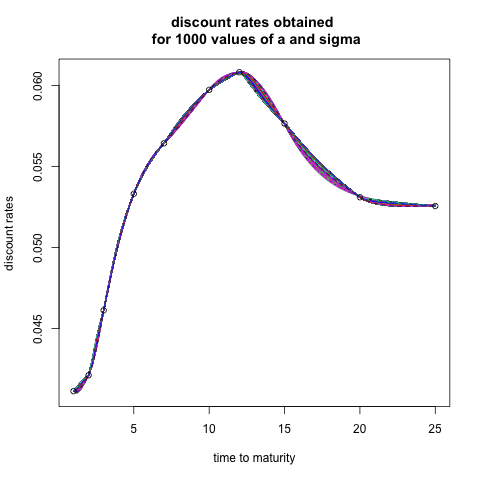
\includegraphics[width=1.065\linewidth, height=0.35\textheight]{gfx/chapter-yc-insurance/construction_graph21}
        \caption{Discount rates obtained for 1000 values of $a \in [0.1, 10]$ and $\sigma \in [0, 0.1]$}
        \label{fig:sensi_a_sigma_1}
    \end{minipage}%
    \begin{minipage}{0.5\textwidth}
        \centering
        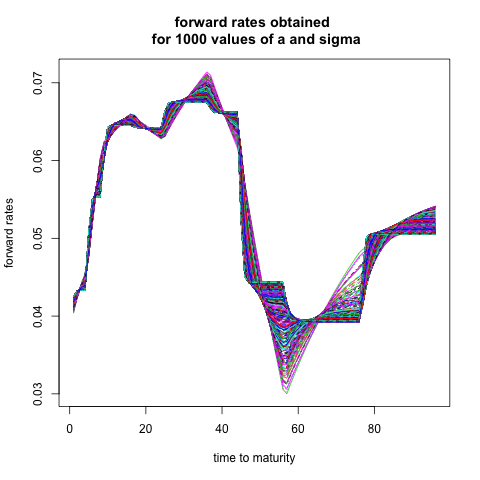
\includegraphics[width=1.065\linewidth, height=0.35\textheight]{gfx/chapter-yc-insurance/construction_graph22}
        \caption{Forward rates obtained for 1000 values of $a \in [0.1, 10]$ and $\sigma \in [0, 0.1]$}
        \label{fig:sensi_a_sigma_2}
    \end{minipage}
  \end{figure}

\subsubsection{Calibration using derivatives}
\label{curvederivatives}

Another way for picking $a$ and $\sigma$ might be to calibrate the underlying short-rate model to a set of caps and swaptions. The optimization procedure would involve the following steps: choosing $a$ and $\sigma$, construct the initial curve with an \textit{exact fit} using the results described in  section \ref{curve_calibration}; use it as an input for theoretical caps and swaptions prices formulas implied by the underlying short-rate model, until $a$ and $\sigma$ which minimize the difference between theoretical and market prices for caps and swaptions are found. 


\subsubsection{Curve extrapolation}
\label{curveextrap}

Using the Hull and White extended Vasicek model, it is possible to derive the instantaneous forward rates from the discount factors formula. We can write:

\begin{equation}
f(0, t) = -\frac{\partial log(P(0,t)}{\partial t} =  X_0e^{-at} + a \int_0^t e^{-a(t-u)}b(u)du-\frac{\sigma^2}{2}\phi^2(t)
\end{equation}

Hence, in our framework, using the fact that $t \mapsto b(t)$ is piecewise constant, we can also write:
\begin{equation}
f^M(0, t) = X_0e^{-at} + a \sum_{i = 1}^n b_i \left[\phi(t-T_{i-1} \wedge t) - \phi(t-T_i \wedge t)\right]+ab_{n+1}\phi(t-T_n \wedge t)-\frac{\sigma^2}{2}\phi^2(t)
\end{equation}
This formula directly provides an input for the simulation of Hull \& White short-rate, with parameters $a$, $\sigma$ and $b_1, \ldots, b_n$ previously calibrated to market data.

\medskip

Hence, let $t$ grow to $\infty$, we have:
\begin{equation}
f^M(0, \infty) = b_{n+1}-\frac{\sigma^2}{2a^2}
\end{equation}

If we assume that the UFR is exogenously chosen, and denote it by $f_\infty$, we are able to derive the parameter $b_{n+1}$ as:

\begin{equation}
b_{n+1} = f_\infty + \frac{\sigma^2}{2a^2}
\end{equation}

This enables to re-write equation (\ref{Intb}), when extrapolation is required, as:

\begin{equation}
\label{Intbbis}
I_{n+1}(t) = \sum_{k=1}^n b_k \left( \xi(t - T_{k-1} \wedge t) -  \xi(t - T_k \wedge t) \right) + \left(f_\infty + \frac{\sigma^2}{2a^2} \right) \xi(t - T_n \wedge t)
\end{equation}

If \textbf{a fixed \textit{ultimate forward rate} (UFR) is defined exogenously}, one can increase or decrease the parameter $a$, to achieve a convergence of $f^M(0, t)$ to $f_\infty$ at a pre-specified maturity. A period of convergence $\tau_{cv}$ after the  \textit{Last Liquid Point} (LLP) is defined. Starting from a low value such as $a = 0.1$, $a$ is increased until:
$$
f^M(0, LLP+\tau_{cv}) = f_\infty
$$
or
$$
|f^M(0, LLP+\tau_{cv}) - f_\infty| < tol
$$
for a given $\sigma$, and a given numerical tolerance $tol$.

\medskip

Otherwise, an \textbf{\textit{ultimate forward rate} (UFR) can be derived from market data}. A static discount curve is fitted to a fraction of the quoted swaps available, called the \textit{training} set. After the construction of the curve on this fraction of the data, we evaluate how well, when extrapolated to a given exogenous UFR, it would price the remaining swaps in a \textit{test} set.

\medskip

The LLP provided by the prudential authority (as of 2016, a maturity 20 years), could be used to define the frontier between the \textit{training} and \textit{test} set. Otherwise,  one can define a percentage of the swaps data to be used as a \textit{training} dataset, for example 80\% or 90\% of the available swaps.

\medskip

Both of these methods for curve extrapolation are applied in the numerical examples, in section \ref{numericalexamples}.

\section{Forecasting with Functional PCA}
\label{curvesforecast}

The idea that a few principal components explain a major part of the changes in bonds returns originates from \cite{litterman1991volatility}. This idea is now well accepted and applied to yield curve forecasting; the interested reader could refer to \cite{diebold2006forecasting} or \cite{christensen2011affine} for example.

\medskip

We use a similar rationale, but apply it somewhat differently. The changes in the swap curve over time, are explained by the changes observed in the calibrated parameters $b_i$s over time. Considering the fact that our model for fitting each cross section of yields is already \textit{overparametrized} (as it uses at least as much parameters as swap rates available in the input dataset), the use of models such as an unrestricted Vector Autoregressive (VAR) to predict the $b_i$s could lead to poor forecasts, with high variance.

\medskip

Functional Principal Components Analysis in the spirit of \cite{ramsay1991some} and \cite{ramsay2005springer}, and more precisely Functional Principal Components Regression, was hence seen as one of the most immediate candidate to achieve a reduction of the problem's dimension. This method is used for example by \cite{hyndman2007robust} for forecasting log mortality rates. It has also been applied in finance, for example in \cite{Benko2007Functional}. 

\medskip

We consider functional data of the form:

\begin{equation}
b^{a, \sigma}_x(t)
\end{equation}

These are the parameters $b_i$s obtained by fitting each cross section of swap rates; observed at increasing times $t \in \left\lbrace t_1, \ldots, t_N \right\rbrace$, for increasing maturities $x \in \left\lbrace x_1, \ldots, x_p \right\rbrace$. The calibration method is the one  described in section \ref{curve_calibration}, with $a$ and $\sigma$ kept fixed over time.

\medskip

\textbf{Finding the Functional Principal Components}

\medskip

Using the approach described in details in \cite{ramsay2005springer}, we let $\textbf{B}$ be the matrix containing at line $i$ and column $j$:
\begin{equation}
\textbf{B}_{i,j} = b^{a, \sigma}_{x_j}(t_i)
\end{equation}

With $i = 1, \ldots, N$ and $j = 1, \ldots, n$, $n > p$. For each cross section of $b_i$s calibrated at time $t_i$, a cubic spline interpolation is applied to $x \mapsto b^{a, \sigma}_{x}(t_i)$, so that the $b_i$s values are now equally spaced on a larger grid of maturities spanning $\left[ x_1, x_p\right]$. Let $w$ be the fixed interpolation step applied to $x \mapsto b^{a, \sigma}_{x}(t_i)$ on $\left[ x_1, x_p\right]$, and:
\begin{equation}
\textbf{V} = \frac{1}{N}\textbf{B}^T\textbf{B}
\end{equation}

$\textbf{V}$ is the covariance matrix of the $b_i$'s, when we consider that the columns of $\textbf{B}$ have been centered. We are then looking for the vectors $\xi^{a, \sigma}$, the (approximate) functional principal components, verifying:
\begin{equation}
w\textbf{V}\xi^{a, \sigma} = \rho \xi^{a, \sigma}
\end{equation}

This is equivalent to searching the eigenvalues and eigenvectors of $\textbf{V}$, so that:
\begin{equation}
\textbf{V} u = \lambda u
\end{equation}
and $\rho = w \lambda$. This problem of finding eigenvalues and eigenvectors of $\textbf{V}$ is typically solved by using the Singular Value Decomposition (SVD) of \textbf{B}, and taking the normalized right singular vectors as functional principal components. The interested reader can refer to \cite{jolliffe2002principal} and \cite{ramsay2005springer} for details. Another interesting resource on Functional Principal Component Analysis is \cite{shang2014survey}.

\medskip

\textbf{Forecasting using Principal Components regression}

\medskip

Having obtained the functional principal components, a least squares regression of the cross sections of $b_i$s is carried out. The $b_i$s are expressed as a linear combination of the previously constructed functional principal components, plus an error term:
\begin{equation}
\forall t \in \left\lbrace t_1, \ldots, t_N \right\rbrace, \: b^{a, \sigma}_{x}(t) = \beta_{t, 0} + \sum_{k = 1}^K \beta_{t, k} \xi^{a, \sigma}_k(x) + \epsilon_t(x)
\end{equation}

$K$ is the number of functional principal components. These functional principal components are not highly correlated by construction, so that we can use univariate time series forecasts for each of the $K+1$ time series, and h-step ahead forecasts of the $b_i$s as:

\begin{equation}
\hat{b}^{a, \sigma}_{x}(t+h) = \hat{\beta}_{t+h|t, 0} + \sum_{k = 1}^K \hat{\beta}_{t+h|t, k} \xi^{a, \sigma}_k(x)
\end{equation}

\medskip

Once the forecasts $\hat{b}^{a, \sigma}_{x}(t+h)$ are obtained, they can be plugged into formulae from section \ref{calibr_bi} to deduce h-step ahead forecasts for the discount factors and discount rates.

\medskip

For choosing \textit{good} values for $a$, $\sigma$ and $K$, we typically used a cross-validation on grids of values for these three parameters, and rolling origin estimation/forecasting, as described in section \ref{numericalexamples}.

\section{Numerical examples}
\label{numericalexamples}

In order to illustrate how the methods described in the previous sections work, we use IRS and OIS data from \cite{andersen2007discount}, \cite{andersen2010interest}, \cite{ametrano2013everything}, an example of bonds data from \cite{hagan2006interpolation}; \textit{a curve where all cubic splines produce negative forward rates}. For forecasting the curves, we use market EUR 6M IRS data, (from which we give detailed summaries) with a CRA adjustment equal to $10$bps.

\medskip

For the data from \cite{andersen2010interest}, we assume that the swaps cash-flows payments occur on an annual basis as for OIS. From \cite{ametrano2013everything}, we consider mid quotes from Eonia OIS and 6-month Euribor IRS as of December 11, 2012. These data sets are all reproduced in the appendices.

\medskip

In section \ref{andersen2010examples}, four calibration methods are tested to illustrate section \ref{curve_calibration}. The method proposed in this paper \footnote{Actually applied to Hull \& White model, but which can be applied to other short-rate models.} is denoted by CMN. It is compared to two iterative curve calibration methods, with linear (LIN) and natural cubic splines (SPL) interpolation on missing dates, and the \cite{smithwilson2001} method (SW). Section \ref{andersen2007examples} also illustrates \ref{curve_calibration}. We use a dataset from \cite{andersen2007discount}; a direct \textit{bootstrapping} without regularization produces wiggly spot and forward rates. The effects of the regularization of approximate second derivative for forward rates and calibrated $b_i$'s is illustrated. Such a regularization could also be applied to noisy bonds data.

\medskip

In section \ref{curvehagan}, the interpolation method is tested on a \textit{curve where all cubic methods produce negative forward rates}, from \cite{hagan2006interpolation}. Section \ref{curveextrapexamples} illustrates the possible extrapolation methods described in  section \ref{curveextrap}. \ref{forecastexample} illustrates the curves' forecasting method introduced in section \ref{curvesforecast}.

\medskip

The discount factors usually display no particular subtleties, so they are deliberately omitted. We present discount rates and discrete forwards instead, and the discrete forwards are taken to be 3-month forward rates.

\subsection{Curve calibration}

\subsubsection{On swaps data from \cite{andersen2010interest}}
\label{andersen2010examples}

Below on figures \ref{fig:andersen2010examples1}, \ref{fig:andersen2010examples2}, \ref{fig:andersen2010examples3}, \ref{fig:andersen2010examples4},  are the discount rates and discrete forwards obtained for the four methods described in the previous section; two \textit{bootstrapping} methods, with linear (LIN) and natural cubic splines (SPL) interpolation on missing dates, the \cite{smithwilson2001} method (SW), and the method described in \ref{curve_calibration} with an exact fit, denoted as CMN. The discount rates are presented as a dashed line, and the forward rates as a plain colored line.


\medskip
\begin{figure}[!htb]
    \centering
    \begin{minipage}{.5\textwidth}
        \centering
        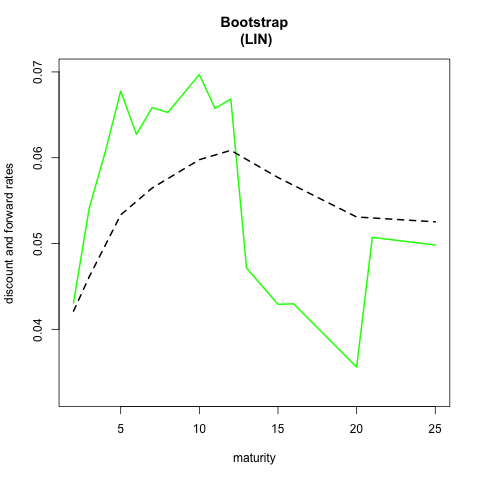
\includegraphics[width=1.06\linewidth, height=0.37\textheight]{gfx/chapter-yc-insurance/construction_graph1}
        \caption{\textit{Bootstrapping} with linear interpolation}
        \label{fig:andersen2010examples1}
    \end{minipage}%
    \begin{minipage}{0.5\textwidth}
        \centering
        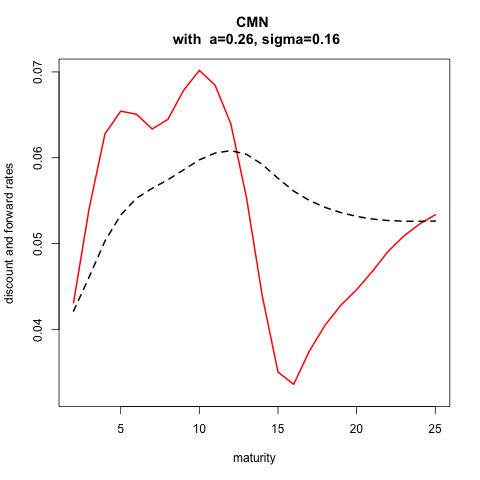
\includegraphics[width=1.06\linewidth, height=0.37\textheight]{gfx/chapter-yc-insurance/construction_graph2}
        \caption{CMN applied to Hull and White extended Vasicek}
        \label{fig:andersen2010examples2}
    \end{minipage}
  \end{figure}

  \begin{figure}[!htb]
        \begin{minipage}{0.5\textwidth}
        \centering
        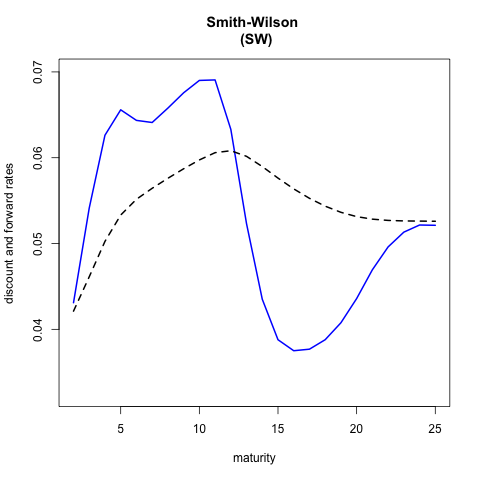
\includegraphics[width=1.06\linewidth, height=0.37\textheight]{gfx/chapter-yc-insurance/construction_graph3}
        \caption{Smith-Wilson method}
        \label{fig:andersen2010examples3}
    \end{minipage}
        \begin{minipage}{0.5\textwidth}
        \centering
        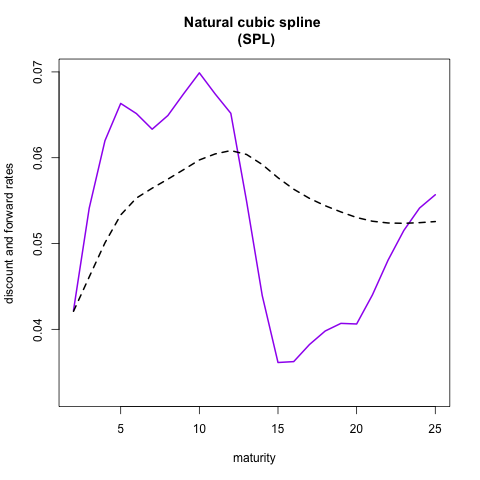
\includegraphics[width=1.06\linewidth, height=0.37\textheight]{gfx/chapter-yc-insurance/construction_graph4}
        \caption{Natural cubic spline}
        \label{fig:andersen2010examples4}
    \end{minipage}
\end{figure}

As demonstrated on figures \ref{fig:andersen2010examples1}, \ref{fig:andersen2010examples2}, \ref{fig:andersen2010examples3} and \ref{fig:andersen2010examples4}, the discount rates produced by the four methods are quite similar. The discrete forward rates better exhibit the differences between them. 

\medskip

Curve construction with linear interpolation between quoted swaps maturities (on figure \ref{fig:andersen2010examples1}), produces a saw-tooth like forward curve, which might not be desirable, and the other methods produce more regular forward curves.

\medskip

For the method described in this paper - denoted as CMN on figure \ref{fig:andersen2010examples2} - and applied to the extended Vasicek model, the discrete forwards (with an exact fit required, as described in section ~\ref{curve_calibration}) reflect the fact that the discount factors' construction relies on a piece-wise constant function, with slight changes in first derivatives at quoted swap maturities. This effect remains very reasonable however, as the discrete forward curve is highly similar to those produced by the other models, and doesn't exhibit large changes at quoted swap maturities.

\medskip

With $a$=\code{0.2557}, $\sigma$=\code{0.1636}, the parameters $b_i$s from table \ref{tab:andersen2010tables1} are obtained. They are presented along with the parameters $\xi_i$s obtained by the method in \cite{smithwilson2001}, with $a = 0.1$. $a = 0.1$ is actually given as default parameter by Solvency II's  technical specifications, and using the notations from QIS5 technical specifications.


\begin{table}[!htb]
\begin{center}
% table caption is above the table
\caption{Parameters obtained for CMN and Smith-Wilson}
\label{tab:andersen2010tables1}       % Give a unique label
% For LaTeX tables use
\begin{tabular}{llllllllll}
\hline\noalign{\smallskip}
Maturity & $b_i$ & $\xi_i$  \\
\noalign{\smallskip}\hline\noalign{\smallskip}
  1 & 0.0661  & -16.680\\
  2 & 0.1894  & 23.556\\
  3 & 0.2523  & -0.8413\\
  5 & 0.2523  & -8.9116\\
  7 & 0.2523  & 3.3552\\
  10 & 0.2806 & 7.9600\\
  12 & 0.2523 & -14.098\\
  15 & 0.2089 & 3.9119\\
  20 & 0.2553 & 3.4828\\
  25 & 0.2616 & -1.9497\\
\noalign{\smallskip}\hline
\end{tabular}
\end{center}
\end{table}

\subsubsection{On noisy swaps data}
\label{andersen2007examples}

This section illustrates what may happen if the method from section ~\ref{curve_calibration} is applied directly to noisy data, without regularization of the parameters. We use data from \cite{andersen2007discount}.

\medskip

Figure \ref{fig:andersen2007examples1} on the left describes the discount and forward rates obtained without regularization, with $a = 0.3655$ and $\sigma =  0.0037$. On the right, figure \ref{fig:andersen2007examples2} describes the discount and forward rates obtained  by minimizing the objective function in equation (\ref{problem3}), and using the parameters $\lambda_1 = 1e-08$ and $\lambda_2 = 1e-05$, $a = 9.8891$ and $\sigma =  0.3957$.

  \begin{figure}[!htb]
    \centering
    \begin{minipage}{.5\textwidth}
        \centering
        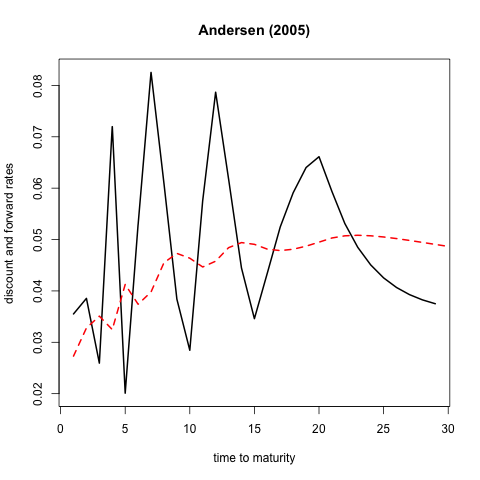
\includegraphics[width=1.05\linewidth, height=0.35\textheight]{gfx/chapter-yc-insurance/construction_graph7}
        \caption{Curve calibration without regularization}
        \label{fig:andersen2007examples1}
    \end{minipage}%
    \begin{minipage}{0.5\textwidth}
        \centering
        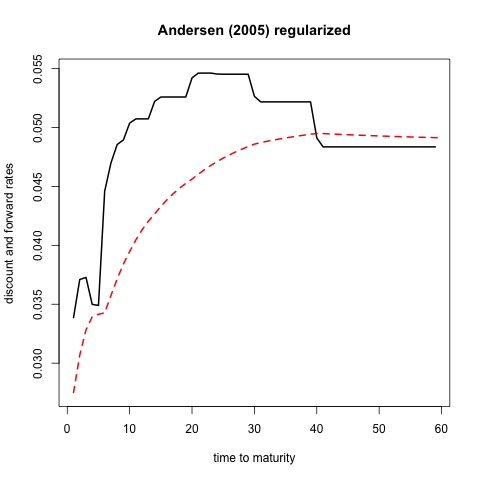
\includegraphics[width=1.05\linewidth, height=0.35\textheight]{gfx/chapter-yc-insurance/construction_graph8}
        \caption{Curve calibration with regularization}
        \label{fig:andersen2007examples2}
    \end{minipage}
  \end{figure}
  
In order to pick $\lambda_1$ and $\lambda_2$, we make a grid search on couples $(\lambda_1, \lambda_2)$. For each $(\lambda_1, \lambda_2)$, a minimization based on derivatives is applied, with multiple restarts of the minimization algorithm. Multiple restarts avoid getting trapped into local minima.

\medskip

Table \ref{tab:andersen2007tables1} contains both the unregularized and regularized $b_i$s. The unregularized ones naturally exhibit a higher variance, because an exact fit to each swap rate in the noisy dataset is required. The regularized $b_i$s exhibit a lower variance, at the expense of a higher bias in the fitting of the data from \cite{andersen2007discount}.

\begin{table}
\begin{center}
% table caption is above the table
\caption{Parameters obtained for unregularized and regularized CMN}
\label{tab:andersen2007tables1}       % Give a unique label
% For LaTeX tables use
\begin{tabular}{llllllllll}
\hline\noalign{\smallskip}
Maturity & unregularized $b_i$ & regularized $b_i$  \\
\noalign{\smallskip}\hline\noalign{\smallskip}
  0.5 & 0.0253  & 0.0281\\
  1 & 0.1100  & 0.0363\\
  1.5 & -0.0078  & 0.0383\\
  2 & 0.0929  & 0.0383\\
  2.5 & -0.0005  & 0.0380\\
  3 & -0.1360  & 0.0352\\
  4 & 0.2901  & 0.0358\\
  5 & 0.1975  & 0.0478\\
  7 & 0.1654  & 0.0497\\
  10 & -0.0056 & 0.0515\\
  12 & 0.1315 & 0.0533\\
  15 & 0.1392 & 0.0554\\
  20 & 0.0688 & 0.0553\\
  30 & 0.039 & 0.0491\\
\noalign{\smallskip}\hline
\end{tabular}
\end{center}
\end{table}

\subsubsection{On \textit{a curve where all cubic methods produce negative forward rates}, with data from \cite{hagan2006interpolation}}
\label{curvehagan}

The dataset from this section is used in \cite{hagan2006interpolation}, and is described as \textit{a curve where all cubic methods produce negative forward rates}. It is reproduced in the appendices.

\medskip

Figure \ref{fig:hagan2006examples1} illustrates the discount rates (dashed line), and discrete forward rates (plain coloured line) obtained with a linear interpolation of the bond yields. The discrete forward remain positive on all maturities, but again exhibit a sawtooth profile. As expected, the natural cubic spline on figure \ref{fig:hagan2006examples2} produces negative discrete forward rates on this dataset.

\begin{figure}[!htb]
    \centering
    \begin{minipage}{.5\textwidth}
        \centering
        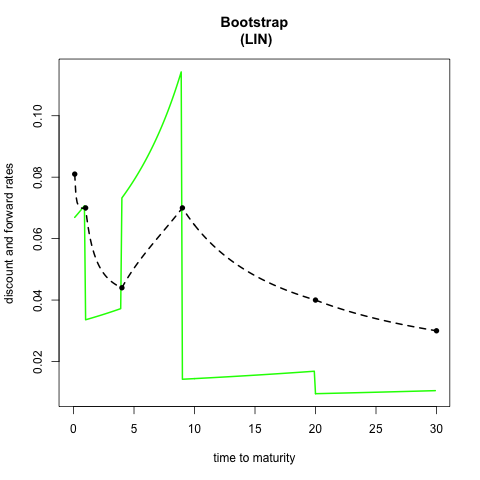
\includegraphics[width=1.06\linewidth, height=0.285\textheight]{gfx/chapter-yc-insurance/construction_graph13}
        \caption{Linear interpolation on \textit{a curve where all cubic methods produce negative forward rates}}
        \label{fig:hagan2006examples1}
    \end{minipage}%
    \begin{minipage}{0.5\textwidth}
        \centering
        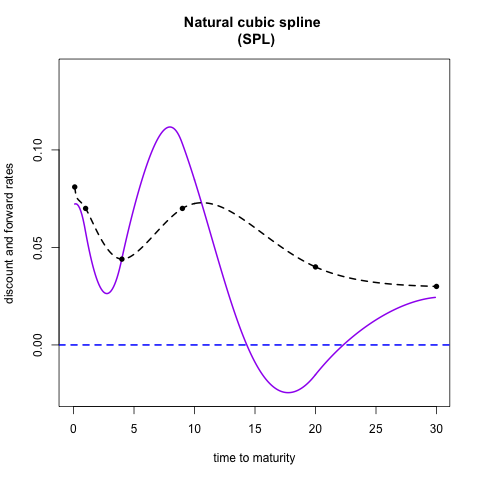
\includegraphics[width=1.06\linewidth, height=0.285\textheight]{gfx/chapter-yc-insurance/construction_graph16}
        \caption{Natural cubic spline interpolation on \textit{a curve where all cubic methods produce negative forward rates}}
        \label{fig:hagan2006examples2}
    \end{minipage}
  \end{figure}
  
  
\begin{figure}[!htb]
    \centering
    \begin{minipage}{.5\textwidth}
        \centering
        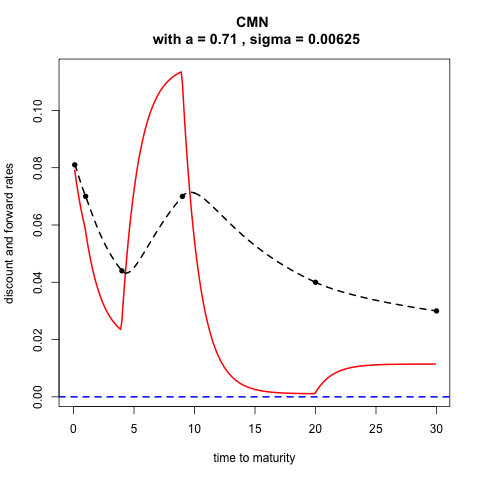
\includegraphics[width=1.06\linewidth, height=0.35\textheight]{gfx/chapter-yc-insurance/construction_graph14}
        \caption{CMN interpolation on \textit{a curve where all cubic methods produce negative forward rates}}
        \label{fig:hagan2006examples3}
    \end{minipage}%
    \begin{minipage}{0.5\textwidth}
        \centering
        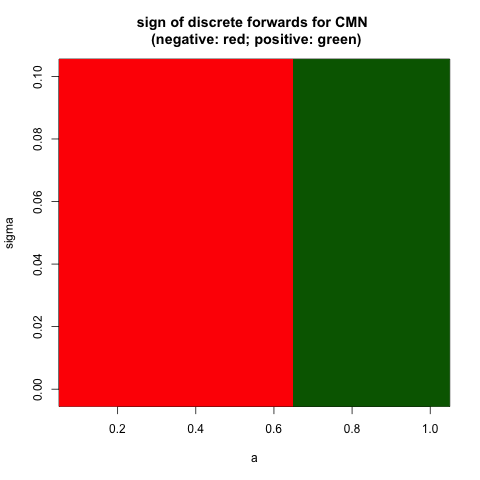
\includegraphics[width=1.06\linewidth, height=0.35\textheight]{gfx/chapter-yc-insurance/construction_graph17}
        \caption{Sign of discrete forwards for CMN as function of $a$ and $\sigma$, on \textit{a curve where all cubic methods produce negative forward rates}}
        \label{fig:hagan2006examples4}
    \end{minipage}
  \end{figure}
  
Figures \ref{fig:hagan2006examples3} and \ref{fig:hagan2006examples4} present the results obtained on data from \cite{hagan2006interpolation}. Figure \ref{fig:hagan2006examples4} presents the sign of discrete forward rates as a function of $a$ and $\sigma$. We consider that discrete forward rates' sign is negative if a least one discrete forward rate is negative. We observe on both figures \ref{fig:hagan2006examples3} and \ref{fig:hagan2006examples4} that a low value of $a$ might produce negative forward rates on maturities comprised between $15$ and $20$. But a high value always produces positive forward rates.

\medskip

This is explained by what we saw in section \ref{curveextrap}: in the Hull and White extend Vasicek case, $a$ controls the speed of convergence of forward rates to the UFR: the higher the $a$, the faster the convergence of forward rates to the UFR on long-term maturities. The parameters obtained by CMN interpolation (for producing figure \ref{fig:hagan2006examples3}), with $a = 0.71$ and $\sigma = 0.0062$ are presented in table \ref{tab:hagan2006tables1}.

\begin{table}[!htb]
\begin{center}
% table caption is above the table
\caption{Parameters obtained CMN with $a = 0.71$ and $\sigma = 0.0062$ on \cite{hagan2006interpolation} data}
\label{tab:hagan2006tables1}       % Give a unique label
% For LaTeX tables use
\begin{tabular}{llllll}
\hline\noalign{\smallskip}
Maturity & $b_i$  \\
\noalign{\smallskip}\hline\noalign{\smallskip}
  0.1 & 0.0718\\
  1 & 0.0351  \\
  4 & 0.0018 \\
  9 & 0.1162  \\
  20 & 0.0011\\
  30 & 0.0114\\
\noalign{\smallskip}\hline
\end{tabular}
\end{center}
\end{table}

\subsection{Curve extrapolation on data from \cite{ametrano2013everything}}
\label{curveextrapexamples}

In this section, we use the extrapolation methods described in \ref{curveextrap}, on OIS and IRS (with CRA adjustment equal to $10$bps) data from \cite{ametrano2013everything}.

\subsubsection{With Solvency II technical specifications, on IRS + CRA}

Extrapolation to a fixed UFR equal to $4.2\%$ is tested, using CMN and the Smith-Wilson method. For both methods, the Last Liquid Point (LLP) is equal to 20 years, and convergence to the UFR is forced to 40 years after the LLP.

\medskip

For the CMN method, the parameters are $a = 0.174$ and $\sigma = 0.0026$, and for the Smith-Wilson method,  $a = 0.125$. The resulting discount and forward curves are presented in figures \ref{fig:extrapCMNSII1} and \ref{fig:extrapSWSII1}, and the parameters $b_i$s and $\xi_i$s in table \ref{tab:ametrano2013tables1}.

\begin{figure}[!htb]
    \centering
    \begin{minipage}{.5\textwidth}
        \centering
        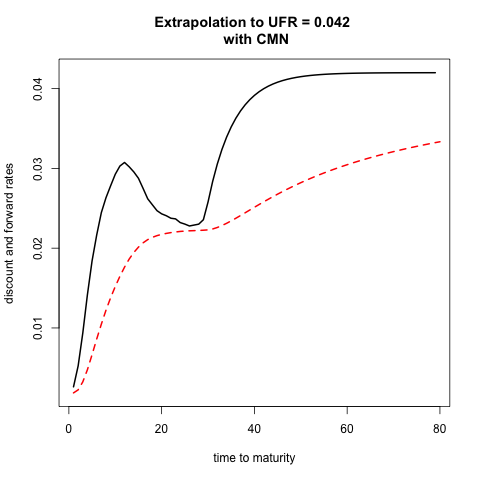
\includegraphics[width=1.065\linewidth, height=0.4\textheight]{gfx/chapter-yc-insurance/construction_graph18}
        \caption{Extrapolation to $UFR = 4.2\%$ with CMN}
        \label{fig:extrapCMNSII1}
    \end{minipage}%
    \begin{minipage}{0.5\textwidth}
        \centering
        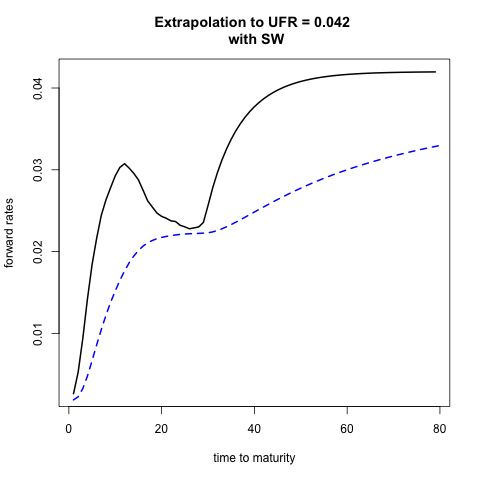
\includegraphics[width=1.065\linewidth, height=0.4\textheight]{gfx/chapter-yc-insurance/construction_graph19}
        \caption{Extrapolation to $UFR = 4.2\%$ with Smith-Wilson}
        \label{fig:extrapSWSII1}
    \end{minipage}
  \end{figure}

\begin{table}
\begin{center}
% table caption is above the table
\caption{Parameters for CMN ($b_i$) and Smith-Wilson ($\xi_i$) extrapolation}
\label{tab:ametrano2013tables1}       % Give a unique label
% For LaTeX tables use
\begin{tabular}{llllllllllllllllllllllllllllll}
\hline\noalign{\smallskip}
Maturity & $b_i$ & $\xi_i$  \\
\noalign{\smallskip}\hline\noalign{\smallskip}
  1 & 0.0019  & -2.5888\\
  2 & 0.0112  & 0.7585\\
  3 & 0.0266  & 0.1415\\
  4 & 0.0352  & 1.3153\\
  5 & 0.0438  & 0.4726\\
  6 & 0.0378  & -0.8809\\
  7 & 0.0399  & 1.2010\\
  8 & 0.0387  & -0.8965\\
  9 & 0.0338  & -0.3536\\
  10 & 0.0376 & 0.7268\\
  11 & 0.0363 & -0.1582\\
  12 & 0.0353 & 1.2852\\
  13 & 0.0312 & -1.9866\\
  14 & 0.0239 & 0.4161\\
  15 & 0.0285 & 0.7056\\
  16 & 0.0211 & -0.7112\\
  17 & 0.0208 & -1.7105\\
  18 & 0.0182 & 1.9922\\
  19 & 0.0248 & -1.5542\\
  20 & 0.0172 & 0.5125\\
  21 & 0.0272 & 1.0148\\
  22 & 0.0189 & -2.1158\\
  23 & 0.0025 & 3.4051\\
  24 & 0.0021 & -3.7822\\
  25 & 0.0020 & 2.7013\\
  26 & 0.0239 & -2.8668\\
  27 & 0.0195 & 2.2513\\
  28 & 0.0274 & -0.8877\\
  29 & 0.0202 & -7.1463\\
  30 & 0.0326 & 8.5322\\
\noalign{\smallskip}\hline
\end{tabular}
\end{center}
\end{table}

\medskip

The discount and forward curves produced by both methods are similar, as seen on figures \ref{fig:extrapCMNSII1} and \ref{fig:extrapSWSII1}. The convergence of the Smith-Wilson method to the UFR seems to be slighty faster. This is caused by the fact that for CMN, we use instantaneous forward rates to assess the convergence to the UFR, whereas for the Smith-Wilson method, we use discrete forwards.

\subsubsection{With OIS data, and a data driven UFR}

For this example, we use OIS data from \cite{ametrano2013everything} presented in the appendices. A training set containing 14 swap rates ($90\%$ of the dataset) with increasing maturities starting at $1$ and ending at $20$ is made up. 

\medskip

This training set is used to construct the discount curve, which is then extrapolated to $30$-year maturity and beyond, using different values for the UFR. The two remaining swaps, with maturities equal to $25$ and $30$, are placed into the test set.

\begin{figure}[!htb]
    \centering
    \begin{minipage}{.5\textwidth}
        \centering
        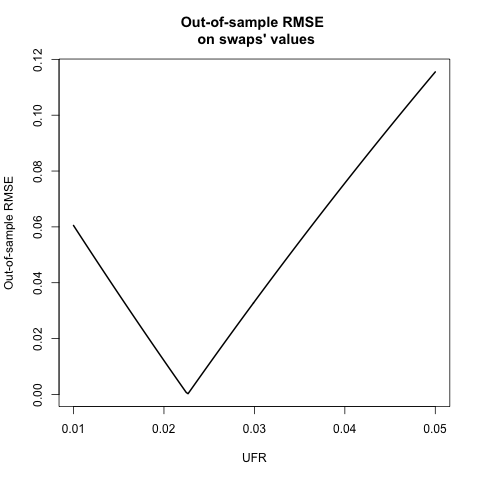
\includegraphics[width=1.06\linewidth, height=0.35\textheight]{gfx/chapter-yc-insurance/construction_graph20_1}
        \caption{Out-of-sample RMSE on swap values, as a function of UFR}
        \label{fig:datadrivenUFR1}
    \end{minipage}%
    \begin{minipage}{0.5\textwidth}
        \centering
        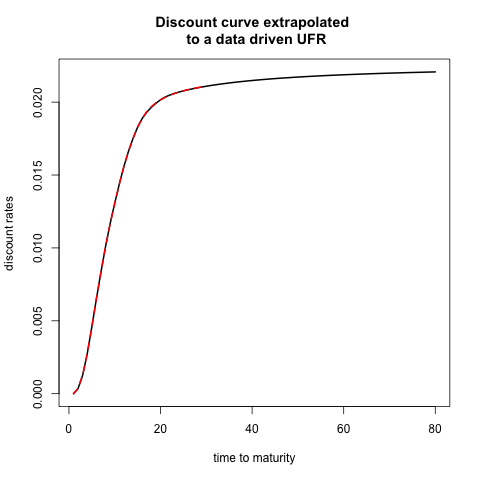
\includegraphics[width=1.06\linewidth, height=0.35\textheight]{gfx/chapter-yc-insurance/construction_graph20_2}
        \caption{Extrapolation of OIS curve to a data driven $UFR = 0.0226$}
        \label{fig:datadrivenUFR2}
    \end{minipage}
  \end{figure}
  
Figure \ref{fig:datadrivenUFR1} presents the out-of-sample RMSE obtained on swaps values from the  test set, as a function of UFR. This error decreases until $UFR = 0.0226$ (notice that this value would depend on the step chosen on the grid of UFRs), and then, starts to increase again. Figure \ref{fig:datadrivenUFR2} displays the discount curve constructed on the training set, extrapolated to a 80-year maturity with an UFR equal to $0.0226$ (the one minimizing the out-of-sample RMSE on the chosen grid of UFRs) is presented.

\subsection{12-months ahead forecast on historical IRS + CRA}
\label{forecastexample}

In this section, we apply ideas from section \ref{curvesforecast} to real world IRS data observed monthly from december 2013 to april 2016, adjusted from a CRA equal to $10$bps.

\medskip

Figure \ref{fig:forecast1} and table \ref{tab:realdatatables1} are to be read together. They  contain the informations on the spot rates derived from the IRS data adjusted from a CRA, using CMN with $a = 0.3655$ and $\sigma = 0.0037$ (other values than $a = 0.3655$ and $\sigma = 0.0037$ would produce the same results as the fitting is exact for many different values of these parameters).

\medskip

The static curves are generally upward sloping, and as time passes, lower and lower spot rates are encountered. In addition, negative rates are observed in table \ref{tab:realdatatables1}; which is coherent with the current context.

\begin{figure}[!htb]
\centering
% Use the relevant command to insert your figure file.
% For example, with the graphicx package use
  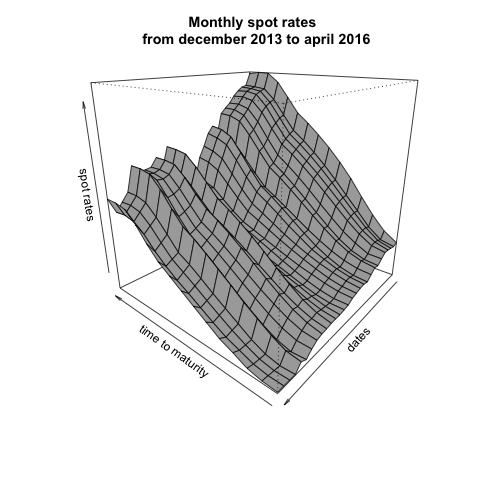
\includegraphics[width=0.75\textwidth]{gfx/chapter-yc-insurance/forecasting_graph1}
% figure caption is below the figure
\caption{Spot rates observed from december 2013 to april 2016}
\label{fig:forecast1}       % Give a unique label
\end{figure}

\begin{table}
\begin{center}
% table caption is above the table
\caption{Descriptive statistics for the spot rates observed from december 2013 to april 2016}
\label{tab:realdatatables1}       % Give a unique label
% For LaTeX tables use
\begin{tabular}{lllllll}
\hline\noalign{\smallskip}
Maturity & Min. & 1st Qrt & Median & Mean & 3rd Qrt & Max.\\
\noalign{\smallskip}\hline\noalign{\smallskip}
  1  & -0.0026 & -0.0008 & 0.0000 & 0.0003  & 0.0019  & 0.0031\\
  3  & -0.0023 & 0.0002  & 0.0009 & 0.0013  & 0.0028  & 0.0065\\
  5  & -0.0008 & 0.0017  & 0.0030 & 0.0037  & 0.0056  & 0.0117\\
  10 & 0.0046  & 0.0059  & 0.0090 & 0.0101  & 0.0132  & 0.0211\\
  15 & 0.0063  & 0.0097  & 0.0127 & 0.0141  & 0.0179  & 0.0258\\
  20 & 0.0069  & 0.0113  & 0.0144 & 0.0157  & 0.0199  & 0.0272\\
  30 & 0.0071  & 0.0118  & 0.0155 & 0.0164  & 0.0208  & 0.0270\\
\noalign{\smallskip}\hline
\end{tabular}
\end{center}
\end{table}

\subsubsection{Benchmarking the model}
\label{benchmarking}

\begin{table}
\begin{center}
% table caption is above the table
\caption{Average out-of-sample error on real world IRS data + CRA}
\label{tab:benchmarktables1}       % Give a unique label
% For LaTeX tables use
\begin{tabular}{llllll}
\hline\noalign{\smallskip}
Method & Parameters  & Avg. OOS error  \\
\noalign{\smallskip}\hline\noalign{\smallskip}
  CMN - \code{auto.arima} & $K = 5$, $a = 1$, $\sigma = 0.1555$ & 0.0031\\
  CMN - \code{ets} & $K = 5$, $a = 1$, $\sigma = 0.2$ & 0.0037 \\
\hline\noalign{\smallskip}
  NS - \code{auto.arima} & $\lambda = 1.8889$ & 0.0031\\
  NS - \code{ets} & $\lambda = 1.8889$ & 0.0035 \\
\hline\noalign{\smallskip}
  NSS - \code{auto.arima} & $\lambda_1 = 21$, $\lambda_2 = 21$ & 0.0027\\
  NSS - \code{ets} & $\lambda_1 = 7$, $\lambda_2 = 3$ & 0.0035 \\
\noalign{\smallskip}\hline
\end{tabular}
\end{center}
\end{table}

Benchmarks are subjective. The one presented in this section does not aim at showing that one method is always superior to the other. It aims at showing that the method presented in this paper produces forecasts which are (more than) reasonable, and actually close to other well-known methods forecasts (on this given dataset).

\medskip

Forecasts from the model presented in section \ref{curvesforecast} are hence compared to those of two other models constructed in the spirit of by the \cite{diebold2006forecasting}. The cross sections of yields described by figure \ref{fig:forecast1} and table \ref{tab:realdatatables1} are fitted by the \cite{nelson1987parsimonious} model (NS), and its extension by \cite{svensson1994estimating} (NSS). The formulas for the spot rates from these models are respectively:

\begin{equation}
\label{NSyield}
R^M(t, T) = \beta_{t, 1} + \beta_{t, 2} \left[ \frac{1 - e^{-T/\lambda}}{T/\lambda}\right] + \beta_{t, 3} \left[ \frac{1 - e^{-T/\lambda}}{T/\lambda} - e^{-T/\lambda} \right]
\end{equation}

and

\begin{eqnarray}
R^M(t, T) &=& \beta_{t, 1} + \beta_{t, 2} \left[ \frac{1 - e^{-T/\lambda_1}}{T/\lambda_1}\right] + \beta_{t, 3} \left[ \frac{1 - e^{-T/\lambda_1}}{T/\lambda_1} - e^{-T/\lambda_1} \right] \\
&+&\beta_{t, 4} \left[ \frac{1 - e^{-T/\lambda_2}}{T/\lambda_2} - e^{-T/\lambda_2} \right]
\end{eqnarray}

Forecasts $\hat{R}^M(t+h, T)$ are obtained by fitting univariate time series to the parameters $\beta_{t, i}, i = 1, \ldots, 4$ with automatic ARIMA (\code{auto.arima}) and exponential smoothing (\code{ets}) models from \cite{hyndman2008automatic}. This automatic selection is done only for the sake of the benchmarking exercise, and in order to conduct the experience in fairly similar conditions for all the methods. In practice, a visual inspection and an actual study of the univariate time series would of course be required.

\medskip

For all the methods the six methods, CMN, NS, NSS with \code{auto.arima} and \code{ets}, we obtain 12-months ahead forecasts, from rolling estimation windows of a fixed 6 months length, starting in december 2013. That is, the models are trained on 6 months data, and predictions are made on 12 months data; successively. The average out-of-sample RMSE are then calculated for each method, on the whole surface of observed and forecasted yields.

\medskip

The \textit{best} parameters for CMN are obtained by cross-validation, with $K \in \left\lbrace 2, 3, 4, 5, 6\right\rbrace$, $5$ values of $a$ comprised between $0.9$ and $1$, and $10$ values of $\sigma$ comprised between $0$ and $0.2$. For NS and NSS, $\lambda_1$ and $\lambda_2$ are chosen by cross-validation, using the rolling estimation/forecasting we have just described.
\subsubsection{Bootstrap simulation of 12-months ahead spot rates}

In this section, we use the last 12 months of the dataset to construct the functional principal components. Using 12 months as the length of the fixed window for estimation, we get an average out-of-sample RMSE of $0.0026$ (on a smaller number of testing samples than the 6 months estimation window, of course).

\medskip

An AR(1) is fitted to the observed univariate time series $(\beta_{t, i})_t$, $i = 0, \ldots, K$, with $a = 1$, $\sigma = 0.0089$, and $K = 3$ chosen by cross-validation. The three functional principal components' characteristics are summarized in table \ref{tab:boot1}. We notice that the first functional principal component explains already $99.2415\%$ of the changes in $b_i$s, and the first three functional principal components selected by cross-validation explain $99.9220\%$.

\begin{table}
\begin{center}
% table caption is above the table
\caption{Importance of Principal components}
\label{tab:boot1}       % Give a unique label
% For LaTeX tables use
\begin{tabular}{llll}
\hline\noalign{\smallskip}
Indicator & PC1 & PC2 & PC3 \\
\noalign{\smallskip}\hline\noalign{\smallskip}
  Standard deviation & 0.1286 & 0.2461 & 0.2246\\
  Proportion of variance (in $\%$) & 99.2415 & 0.5489 & 0.1315\\
  Cumulative Proportion (in $\%$) & 99.2415 & 99.7904 & 99.9220\\
\noalign{\smallskip}\hline
\end{tabular}
\end{center}
\end{table}

% \begin{figure*}[!htb]
% \centering
% % Use the relevant command to insert your figure file.
% % For example, with the graphicx package use
%   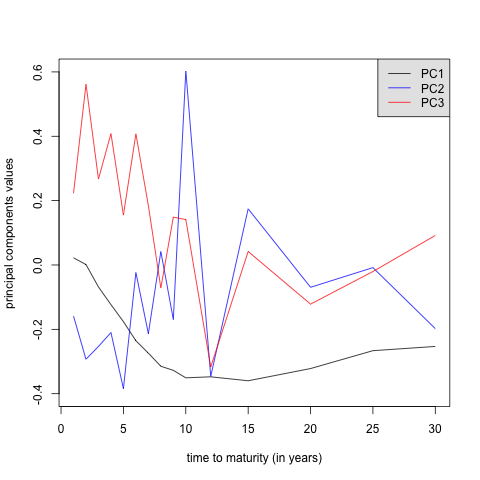
\includegraphics[width=0.6\textwidth]{forecasting_graph5}
% % figure caption is below the figure
% \caption{Principal components of the $b_i$s from april 2015 to april 2016}
% \label{fig:forecast2}       % Give a unique label
% \end{figure*}

\medskip

Figure \ref{forecast:3} presents the autocorrelation functions of the residuals of AR(1)  fitted to $(\beta_{t, i}),  \: i = 0, \ldots, 3$ from april 2015 to april 2016. The residuals from AR(1) fitted to $(\beta_{t, i})_t, \: i = 1, \ldots, 3$ could be considered as stationary, but those from the AR(1) fitted to $(\beta_{t, 0})_t$ seems to be closer to an AR(4).

\medskip

We denote these residuals by $(\epsilon_{t, i})_t, \: i = 0, \ldots, 3$. In order to obtain simulations for the $(\beta_{t, i})_t,  \: i = 0, \ldots, 3$, it is possible to use a Gaussian hypothesis on the residuals. We choose to create one thousand bootstrap resamples with replacement of the $(\epsilon_{t, i})_t, \: i = 0, \ldots, 3$ \footnote{Even if for $\epsilon_{t, 0}$, considering figure \ref{forecast:3}, this makes a strong stationarity assumption on the residuals.}, denoted as $(\epsilon_{t, i}^*)_t, \: i = 0, \ldots, 3$, and create new pseudo values for $(\beta_{t, i}),  \: i = 0, \ldots, 3$:
$$
\beta^*_{t, i} = \beta_{t, i} + \epsilon_{t, i}^*,  \: i = 0, \ldots, 3
$$

\medskip

Having done this, AR(1) forecasts $\beta^*_{t+h|t, i}$ can be obtained, in order to construct:

\begin{equation}
\hat{b}^{a, \sigma, *}_{x}(t+h) = \hat{\beta}^*_{t+h|t, 0} + \sum_{k = 1}^K \hat{\beta}^*_{t+h|t, k} \xi^{a, \sigma}_k(x)
\end{equation}

\medskip

The $\hat{b}^{a, \sigma, *}_{x}(t+h)$ can then be plugged into formulae \ref{la_formule} and \ref{Intb} to deduce simulations of h-step ahead forecasts for the discount factors and discount rates.

\medskip

The simulations (1000) of 12-months ahead discount rates are presented in figures \ref{forecast:4} and \ref{forecast:5}.

\begin{figure}[!htb]
\centering
% Use the relevant command to insert your figure file.
% For example, with the graphicx package use
  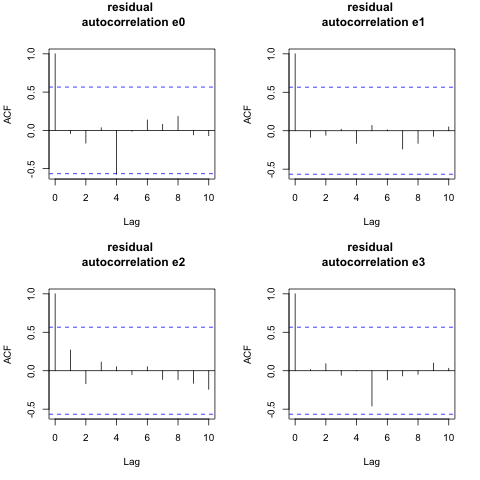
\includegraphics[width=0.85\textwidth]{gfx/chapter-yc-insurance/forecasting_graph2}
% figure caption is below the figure
\caption{Autocorrelation functions for the residuals of univariate time series(AR(1)) on $\beta_0$, $\beta_1$, $\beta_2$, $\beta_3$}
\label{forecast:3}       % Give a unique label
\end{figure}

\begin{figure}[!htb]
    \centering
    \begin{minipage}{.5\textwidth}
        \centering
        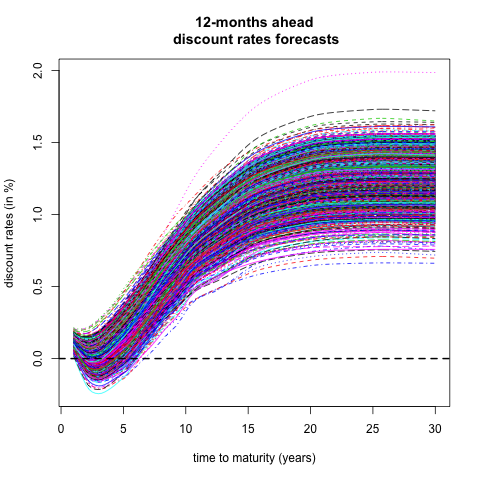
\includegraphics[width=0.8\linewidth, height=0.3\textheight]{gfx/chapter-yc-insurance/forecasting_graph3}
        \caption{Curves simulated with principal components from april 2015 to april 2016, and bootstrap ressampling of the residuals}
        \label{forecast:4}
    \end{minipage}%
    \begin{minipage}{0.5\textwidth}
        \centering
        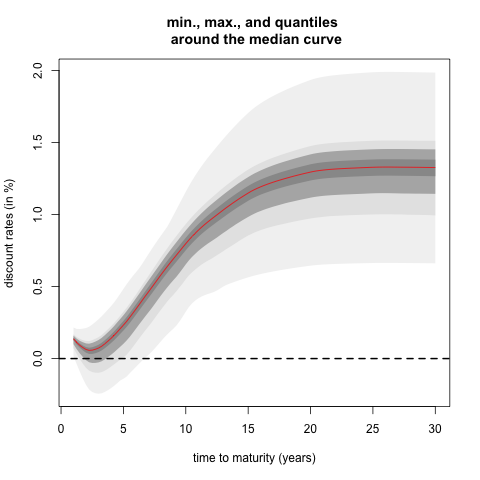
\includegraphics[width=0.8\linewidth, height=0.3\textheight]{gfx/chapter-yc-insurance/forecasting_graph4}
        \caption{Min., Max., and quartiles around the median curve for the simulations}
        \label{forecast:5}
    \end{minipage}
  \end{figure}

\begin{table}
\begin{center}
% table caption is above the table
\caption{Descriptive statistics for fitted parameters $b_i$s from april 2015 to april 2016}
\label{tab:realdatatables2}       % Give a unique label
% For LaTeX tables use
\begin{tabular}{lllllll}
\hline\noalign{\smallskip}
Maturity & Min. & 1st Qrt & Median & Mean & 3rd Qrt & Max.\\
\noalign{\smallskip}\hline\noalign{\smallskip}
  1  & -0.0026 & -0.0021 & -0.0010 & -0.0013 & -0.0004  & -0.0003\\
  3  & 0.0000  & 0.0026  & 0.0040  & 0.0035  & 0.0048  & 0.0058\\
  5  & 0.0025  & 0.0076  & 0.0030  & 0.0092  & 0.0108  & 0.0143\\
  10 & 0.0115  & 0.0174  & 0.0090  & 0.0188  & 0.0208  & 0.0230\\
  15 & 0.0122  & 0.0168  & 0.0127  & 0.0192  & 0.0220  & 0.0228\\
  20 & 0.0117  & 0.0148  & 0.0144  & 0.0171  & 0.0195  & 0.0211\\
  30 & 0.0080  & 0.0116  & 0.0155  & 0.0134  & 0.0150  & 0.0178\\
\noalign{\smallskip}\hline
\end{tabular}
\end{center}
\end{table}

\subsection{6-months and 36-months ahead forecast on longer historical data}
\label{forecastexample2}

In this second example, we use interest rate swaps data from the Federal Reserve Bank of St Louis website \footnote{Available at https://fred.stlouisfed.org/categories/32299} observed monthly, from july 2000 to september 2016, with maturities equal to $1, 2, 3, 4, 5, 7, 10, 30$, and a tenor equal to three months. 

\medskip

In figure \ref{forecast:6}, we represent the eight time series of swap rates, observed for each maturity $1, 2, 3, 4, 5, 7, 10, 30$, between july 2000 and september 2016. The swap rates for different maturities generally exhibit a decreasing trend, and are nearly equal to 0 by the end of 2016 for the shortest maturities. 

\medskip

Starting in 2006, the spreads between swap rates with different maturities start to narrow, until the end of 2007, and swap rates for short maturities are relatively high. This is the period corresponding to the Liquidity and Credit Crunch 2007-2008. Table \ref{tab:freddatatables1} below presents the descriptive statistics for the data. 

%\newpage

\begin{figure}[!htb]
\centering
% Use the relevant command to insert your figure file.
% For example, with the graphicx package use
  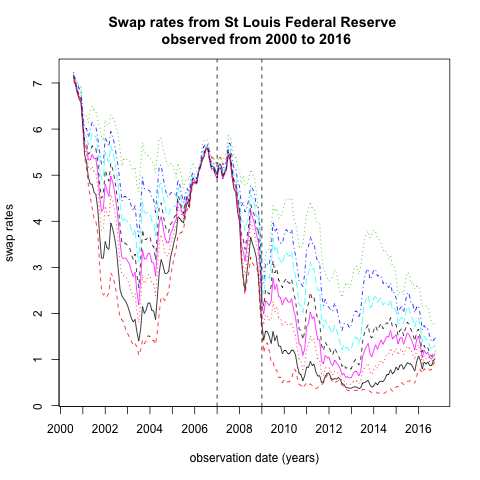
\includegraphics[width=0.75\textwidth]{gfx/chapter-yc-insurance/forecasting_graph6}
% figure caption is below the figure
\caption{Swap rates data (in \%) from St Louis Federal Reserve Bank, at maturities $1, 2, 3, 4, 5, 7, 10, 30$}
\label{forecast:6}       % Give a unique label
\end{figure}


\begin{table}
\begin{center}
% table caption is above the table
\caption{Descriptive statistics for St Louis Federal Reserve data}
\label{tab:freddatatables1}       % Give a unique label
% For LaTeX tables use
\begin{tabular}{lllllll}
\hline\noalign{\smallskip}
Maturity & Min. & 1st Qrt & Median & Mean & 3rd Qrt & Max.\\
\noalign{\smallskip}\hline\noalign{\smallskip}
  1  & 0.0026 & 0.0050  & 0.0134  & 0.0211  & 0.0336  & 0.0705\\
  2  & 0.0037 & 0.0078  & 0.0182  & 0.0239  & 0.0390  & 0.0712\\
  3  & 0.0046 & 0.0108  & 0.0236  & 0.0269  & 0.0422  & 0.0714\\
  4  & 0.0060 & 0.0134  & 0.0280  & 0.0296  & 0.0439  & 0.0715\\
  5  & 0.0078 & 0.0167  & 0.0316  & 0.0319  & 0.0456  & 0.0717\\
  7  & 0.0119 & 0.0215  & 0.0368  & 0.0354  & 0.0483  & 0.0720\\
  10 & 0.0139 & 0.0261  & 0.0419  & 0.0388  & 0.0502  & 0.0724\\
  30 & 0.0175 & 0.0327  & 0.0465  & 0.0440  & 0.0537  & 0.0720\\
\noalign{\smallskip}\hline
\end{tabular}
\end{center}
\end{table}

\medskip

We transformed these swap rates into zero rates by using a single curve calibration (that is, ignoring the counterparty credit risk) with linear interpolation between the maturities; one of the methods used in section ~\ref{andersen2010examples}. Then, as in the previous section, NS, NSS, CMN are used for fitting and forecasting the curves, with \code{auto.arima} applied to the factors. 

\medskip

We obtain 6-months and 36-months ahead forecasts,  from rolling training/testing windows (as in the last section) with respectively, a fixed  6 and 36 months length. The average out-of-sample RMSE are then calculated for each method, on the whole set of observed and forecasted yields. 

\medskip

The \textit{best} hyperparameters - associated with the lowest out-of-sample average RMSE - for each model are obtained through a search on a grid of values. For a 6-months horizon, they are (using the notations from section \ref{benchmarking}):
\begin{itemize}
\item NS: $\lambda = 1.6042$  
\item NSS: $\lambda_1 = 1.6250$ $\lambda_2 = 1.6250$
\item CMN: $a = 177.8279$, $\sigma = 3.9473e-04$, $K = 6$
\end{itemize}

and for a 36-months horizon: 
\begin{itemize}
\item NS: $\lambda = 1.4271$  
\item NSS: $\lambda_1 = 1.575$ $\lambda_2 = 1.575$
\item CMN: $a = 14.6780$, $\sigma = 0.0011$, $K = 4$
\end{itemize}

\medskip

The following results are obtained for the out-of-sample average RMSE: 

\begin{table}[!htb]
\begin{center}
% table caption is above the table
\caption{Descriptive statistics for out-of-sample RMSE, for training window = 6 months, and testing window = 6 months}
\label{tab:freddatatables3}       % Give a unique label
% For LaTeX tables use
\begin{tabular}{llllllll}
\hline\noalign{\smallskip}
Method & Min. & 1st Qrt & Median & Mean & 3rd Qrt & Max. & Std. Dev\\
\noalign{\smallskip}\hline\noalign{\smallskip}
  NS   & 0.00101  & 0.00269  & 0.00409  & 0.00481  & 0.00595  & 0.01530 & 0.00296\\
  NSS  & 0.00102  & 0.00269  & 0.00411  & 0.00481  & 0.00595  & 0.01537 & 0.00296\\
  CMN  & 0.00115  & 0.00256  & 0.00396  & 0.00468  & 0.00580  & 0.01600 & 0.00302\\
\noalign{\smallskip}\hline
\end{tabular}
\end{center}
\end{table}

\begin{table}[!htb]
\begin{center}
% table caption is above the table
\caption{Descriptive statistics for out-of-sample RMSE, for training window = 36 months, and testing window = 36 months}
\label{tab:freddatatables4}       % Give a unique label
% For LaTeX tables use
\begin{tabular}{llllllll}
\hline\noalign{\smallskip}
Method & Min. & 1st Qrt & Median & Mean & 3rd Qrt & Max. & Std. Dev\\
\noalign{\smallskip}\hline\noalign{\smallskip}
  NS   & 0.00356  & 0.00703  & 0.01044  & 0.01489  & 0.01609  & 0.21500 & 0.0213\\
  NSS  & 0.00300  & 0.00690  & 0.01114  & 0.01484  & 0.01689  & 0.21570 & 0.0201\\
  CMN  & 0.00402  & 0.00945  & 0.01279  & 0.01452  & 0.01917  & 0.03710 & 0.0070\\
\noalign{\smallskip}\hline
\end{tabular}
\end{center}
\end{table}

Using tables \ref{tab:freddatatables3}, \ref{tab:freddatatables4} and figures \ref{forecast:7} and \ref{forecast:8}, we observe that CMN give results which are close to those from NS and NSS, with a lower average out-of-sample RMSE in both cases. For a training window equal to six months, and testing window of six months, the results obtained by the three methods are pretty similar, and the same performance is observed for the three during the financial crisis.  For a training and testing window of thirty six months length, CMN has a lower mean and standard deviation for out-of-sample RMSE overall, but doesn't perform the best in the period of financial crisis 2007-2009. 

%\newpage

\begin{figure}[!htb]
\centering
% Use the relevant command to insert your figure file.
% For example, with the graphicx package use
  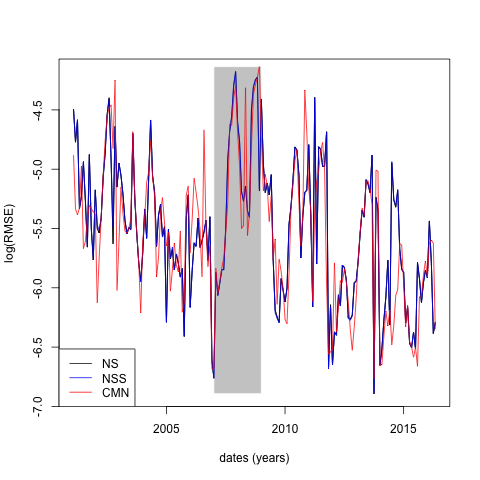
\includegraphics[width=0.65\textwidth]{gfx/chapter-yc-insurance/forecasting_graph7}
% figure caption is below the figure
\caption{log(out-of-sample RMSE) for training window = 6 months, and testing window = 6 months}
\label{forecast:7}       % Give a unique label
\end{figure}

\begin{figure}[!htb]
\centering
% Use the relevant command to insert your figure file.
% For example, with the graphicx package use
  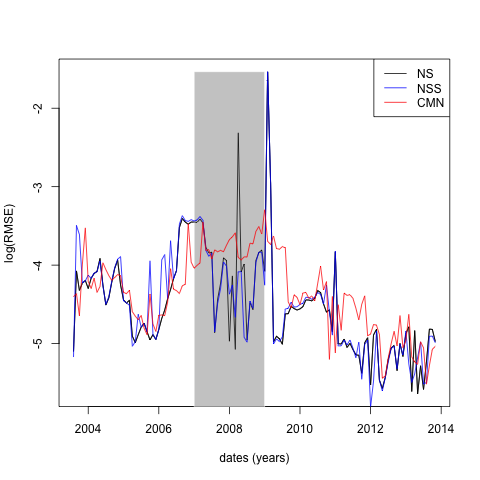
\includegraphics[width=0.65\textwidth]{gfx/chapter-yc-insurance/forecasting_graph8}
% figure caption is below the figure
\caption{log(out-of-sample RMSE) for training window = 36 months, and testing window = 36 months}
\label{forecast:8}       % Give a unique label
\end{figure}

\section{Conclusion}

In this paper, we introduced a method for swap discount curve construction and extrapolation. This method relies on the closed form formulas for discount factors available in exogenous short-rate models. We presented different ways to calibrate and extrapolate the model on different data sets from the existing literature. Moreover, we showed that the model's parameters contain a certain predictive power, enabling to obtain swap curves' forecasts, with predictive distribution.


\newpage

\section{Appendix}

\subsection{Data from \cite{andersen2010interest}}

\medskip
\begin{center}
\begin{tabular}{|l|c|r|}
  \hline
  Maturity & Swap Par Rate \\
  \hline
  1 & 4.20\% \\
  2 & 4.30\%  \\
  3 & 4.70\%  \\
  5 & 5.40\%  \\
  7 & 5.70\%  \\
  10 & 6.00\%  \\
  12 & 6.10\%  \\
  15 & 5.90\%  \\
  20 & 5.60\%  \\
  25 & 5.55\%  \\
  \hline
\end{tabular}
\end{center}

\subsection{Data from \cite{andersen2007discount}}

\medskip
\begin{center}
\begin{tabular}{|l|c|r|}
  \hline
  Maturity & Swap Par Rate \\
  \hline
  0.5 & 2.75\% \\
  1 & 3.10\%  \\
  1.5 & 3.30\%  \\
  2 & 3.43\%  \\
  2.5 & 3.53\%  \\
  3 & 3.30\%  \\
  4 & 3.78\%  \\
  5 & 3.95\%  \\
  7 & 4.25\%  \\
  10 & 4.50\%  \\
  12 & 4.65\%  \\
  15 & 4.78\%  \\
  20 & 4.88\%  \\
  30 & 4.85\%  \\
  \hline
\end{tabular}
\end{center}

\subsection{Data from \cite{hagan2006interpolation}}

\medskip
\begin{center}
\begin{tabular}{|l|c|r|}
  \hline
  Maturity & Continuous yield \\
  \hline
  0.1 & 8.10\% \\
  1 & 7.00\%  \\
  4 & 4.40\%  \\
  9 & 7.00\%  \\
  20 & 4.00\%  \\
  30 & 3.00\%  \\
  \hline
\end{tabular}
\end{center}


\subsection{Data from \cite{ametrano2013everything}}

\medskip
\begin{center}
\begin{tabular}{|l|c|r|}
  \hline
  Maturity & EUR6M IRS & Eonia OIS  \\
  \hline
  1 & 0.286\% & 0.000\% \\
  2 & 0.324\%  & 0.036\% \\
  3 & 0.424\%  & 0.127\% \\
  4 & 0.576\%  & 0.274\% \\
  5 & 0.762\%  & 0.456\% \\
  6 & 0.954\%  & 0.647\% \\
  7 & 1.135\%  & 0.827\% \\
  8 & 1.303\%  & 0.996\% \\
  9 & 1.452\%  & 1.147\% \\
  10 & 1.584\%  & 1.280\% \\
  11 & 1.703\%  & 1.404\% \\
  12 & 1.809\%  & 1.516\% \\
  13 & 1.901\%  & - \\
  14 & 1.976\%  & - \\
  15 & 2.037\%  &  1.764\%\\
  16 & 2.086\%  & - \\
  17 & 2.123\%  & - \\
  18 & 2.150\%  & - \\
  19 & 2.171\%  & - \\
  20 & 2.187\%  & 1.939\% \\
  21 & 2.200\%  & - \\
  22 & 2.211\%  & - \\
  23 & 2.220\%  & - \\
  24 & 2.228\%  & - \\
  25 & 2.234\%  & 2.003\% \\
  26 & 2.239\%  & - \\
  27 & 2.243\%  & - \\
  28 & 2.247\%  & - \\
  29 & 2.251\%  & - \\
  30 & 2.256\%  & 2.038\% \\
  35 & 2.295\%  & - \\
  40 & 2.348\%  & - \\
  50 & 2.421\%  & - \\
  60 & 2.463\%  & - \\
  \hline
\end{tabular}
\end{center}
 % INCLUDE: yc-insurance
\forcenewpage

%% !TEX root = ../thesis-example.tex
%
\chapter{Conclusion}
\label{sec:conclusion}

 % INCLUDE: conclusion
%\cleardoublepage

% --------------------------
% Back matter
% --------------------------
{%
\setstretch{1.1}
\renewcommand{\bibfont}{\normalfont\small}
\setlength{\biblabelsep}{0pt}
\setlength{\bibitemsep}{0.5\baselineskip plus 0.5\baselineskip}
\printbibliography[nottype=online]
\printbibliography[heading=subbibliography,title={Webseiten},type=online,prefixnumbers={@}]
}
\cleardoublepage

\listoffigures
\cleardoublepage

\listoftables
\cleardoublepage

% !TEX root = ../thesis-example.tex
%
\pagestyle{empty}
\hfill
\vfill
\pdfbookmark[0]{Colophon}{Colophon}
\section*{Colophon}

This thesis was typeset with \LaTeXe.
It uses the \textit{Clean Thesis} style developed by Ricardo Langner.
The design of the \textit{Clean Thesis} style is inspired by user guide documents from Apple Inc.

Download the \textit{Clean Thesis} style at \url{http://cleanthesis.der-ric.de/}.

\cleardoublepage

% !TEX root = ../thesis-example.tex
%
%************************************************
% Declaration
%************************************************
\pdfbookmark[0]{Declaration}{Declaration}
\chapter*{Declaration}
\label{sec:declaration}
\thispagestyle{empty}

You can put your declaration here, to declare that you have completed your work solely and only with the help of the references you mentioned.

\bigskip

\noindent\textit{\thesisUniversityCity, \thesisDate}

\smallskip

\begin{flushright}
	\begin{minipage}{5cm}
		\rule{\textwidth}{1pt}
		\centering\thesisName
	\end{minipage}
\end{flushright}

%*****************************************
%*****************************************

\clearpage
\newpage
\mbox{}

% **************************************************
% End of Document CONTENT
% **************************************************
\end{document}
